% The following choice requires a coordinated choice when PRINTING the report:
%\documentclass[oneside,12pt]{report}  % Use this for one-sided copying (print with printer's normal
%  single-sided option
\documentclass[twoside,12pt,openright]{report}  % You can use this for a slim final printed copy (print with 
%  printer's double-sided option)

% the dimensions of the page
\textheight=9.25in \topmargin=-0.5in   %See note in Chapter 8 of Sample Report about "Page scaling" option in Adobe
\textwidth=6.0in
\oddsidemargin=0.3in
\evensidemargin=0.3in  % Needed to balance even and odd pages in twoside print copy

% Useful packages
\usepackage{amsmath}
\usepackage{amsfonts}
\usepackage{amsbsy}

%% In the following, the assumption is that your graphics are in encapsulated postscript (eps).  If not,
%% you may need to use some other method for incorporating graphics into your pdf of the final report.
%  Use the next package for typesetting directly to dvi or postcript (used primarily for the PCTeX typesetter, 
%  see the following alternatives).
\usepackage[dvips]{graphicx} 
% Use the next two packages together for typesetting directly to pdf (this works for pdfLaTeX and may work 
% for others---not yet tested for all---please report your experience).
%\usepackage[pdftex]{graphicx}
%\usepackage{epstopdf}
%%

\usepackage{doc}
% Following sets up logic and formatting for conditional twoside copying
\usepackage{ifthen, color, fancyvrb}
\usepackage{nextpage}\pagestyle{plain}
\newcommand\myclearpage{\cleartooddpage
  [\thispagestyle{empty}]
  }

%  Set font size for captions
\usepackage[skip=4pt,font=footnotesize]{caption}


\DeclareGraphicsExtensions{ps,eps}
\usepackage{excludeonly}

% If some words are being hyphenated incorrectly, they can be
% given in a list to the \hyphenation command as below.
\hyphenation{ap-pen-dix wer-ther-i-an}

\usepackage{amsthm}                % Theorem/proof enviornments.
% Theorem-like command definitions:
\newtheorem{theorem}{Theorem}[chapter]
\newtheorem{lemma}{Lemma}[chapter]
\newtheorem*{definition}{Definition}  % Note, this italicizes everything

% Print the chapter and sections in the toc
\setcounter{tocdepth}{1}

% Specify which files to typeset for this run (note that overall pagination is preserved)
%\includeonly{chapter1, chapter2}

% Specify which files NOT to typeset for this run (note that overall pagination is preserved)
%\excludeonly{}

% Groundwork for allowing double-sided copying with blank versos
\def\prefacesection#1{
\chapter*{#1}
\addcontentsline{toc}{chapter}{#1}
}


\usepackage{amssymb}               % Various symbols.
%\usepackage{geometry}              % Easy interface to set page margins.
%\usepackage{fancyhdr}              % Custom headers/footers, page styles.
\usepackage[shortlabels]{enumitem} % Stuff for enumerate, itemize environments.
\usepackage{tikz}
\usepackage{stmaryrd}
\usepackage{bbm}
\usepackage{latexsym}
\usepackage{graphicx}
\usepackage{subcaption}
\usepackage{algorithm2e}
\usepackage{mathtools}
\usepackage{array}
\usepackage{float}
\newcolumntype{P}[1]{>{\centering\arraybackslash}p{#1}}

%\geometry{margin=3cm}              % Sets margins on all sides.
%\pagestyle{fancyplain}             % Sets page style.
%\headheight 35pt                   % Sets the height of the header.
%\headsep 10pt                      % Sets space between the header and the body.

\setlength{\parindent}{0em}        % Sets paragraph indentation.
\setlength{\parskip}{0.5em}        % Sets space between paragraphs.

\setlist[itemize]{leftmargin=*}    % Normalize left margin in itemize. 
\setlist[enumerate]{leftmargin=*}  % Normalize left margin in enumerate.


\newenvironment{solution}{\textit{Solution.}}
\allowdisplaybreaks


\newcommand\semester{Summer 2018}  
\newcommand\banner{AMD}      
\newcommand\E{\mathbb{E}}

\DeclareMathOperator*{\argmax}{arg\,max}

%\lhead{\banner}
%\chead{\textbf{\Large Final Report}}
%\rhead{\semester}


\begin{document}

% Footnote references are symbolized in the front matter, but see below for restoration of numbered footnotes in the body.
\def\thefootnote{\fnsymbol{footnote}}

% The title page is in its own file, ``titlepage.tex''.
% It needs to be edited to reflect information specific
% to your project. 
% don't display the page number
\thispagestyle{empty}

% The numbers below controls the amount of space between the following sections
\def\shiftdowna{0.32in}  % Adjust for balance
\def\shiftdownb{0.22in}  % Adjust for balance

% Set up the boiler plate at the top of the page
\begin{center}
\textbf{{\large Research in Industrial Projects for Students}}\\

\vspace \shiftdowna
%\includegraphics[width=0.4\textwidth]{ipam.eps}\\

\includegraphics[width=0.4\textwidth]{Graphics/ipamlogo_cmyk_full_lg.eps}\\


% SPONSOR
\vspace \shiftdowna
\underline {Sponsor}\\ 
\vspace{5pt}
 \textbf{\large Advanced Micro Devices}  \\
\vspace \shiftdowna
\textbf{Final Report}

% TITLE
\vspace \shiftdowna
\textbf{{\Large Exploration of Reinforcement Learning in Computer Games}}

% Note the convention used here:  email addresses and urls are typeset in teletype font, colleges are set in italics.

% STUDENTS
\vspace{0.35in}
\underline {Student Members}\\
\vspace{5pt}
\text{Jiajing Guan} (Project Manager),  \text{\emph{George Mason University}}\\ 
\vspace{3pt}
\text{\texttt{jiajingguan@gmail.com}} \\
\vspace{3pt}
\text{Patrik Gerber}, \text{\emph{University of Oxford}}  \\
\vspace{3pt}
\text{Elvis Nunez}, \text{\emph{Brown University}}  \\
\vspace{3pt}
 \text{Kaman Phamdo},  \text{\emph{University of Maryland}}  \\


% ACADEMIC MENTORS
\vspace \shiftdownb
\underline {Academic Mentor} \\
\vspace{5pt}
\text{Tonmoy Monsoor}, \text{\texttt{mtonmoy@g.ucla.edu}} 

% SPONSORS
\vspace \shiftdownb
\underline {Sponsoring Mentors}\\
\vspace{5pt}
\text{Nicholas Malaya},  \text{\texttt{nicholas.malaya@amd.com}} \\
\vspace{3pt}
 \text{Abhinav Vishnu},  \text{\texttt{abhinav.vishnu@amd.com}} \\
\vspace{3pt}
\text{Alan Lee}, \text{\texttt{alan.lee@amd.com}}  \\

% CONSTULANTS (comment out this text if there are no consultants)

% DATE
\vspace \shiftdowna
\text{Date: \today}

\end{center}

\vfill  %Fill page to force following note to bottom
\footnoterule
\noindent \small{This project was jointly supported by \text{Advanced Micro Devices} and NSF Grant  \text{DMS-0931852}.}



% Begin ABSTRACT
\ifthenelse{\boolean{@twoside}}{\myclearpage}{}
\prefacesection{Abstract}
\thispagestyle{empty}


Reinforcement learning (RL) is an area of machine learning where algorithms learn from experience while dynamically interacting with an environment. RL approaches have recently achieved superhuman performance in games such as Go, Chess, and classic video games. However, these algorithms are sensitive to perturbations in the environment and often struggle or catastrophically fail when applied to environments that differ from where they were trained. RL methods must become more robust if they are to become certified and deployed in the real-world. This project investigated the performance of the Deep Q-Network (DQN) algorithm on an unsolved OpenAI car racing game challenge. The report begins with an overview of reinforcement learning and the methods used for the car racing game. This is followed by a description of a tuned DQN algorithm that solves this particular challenge. The algorithm’s sensitivity to changes in feedback and input image characteristics are discussed. This report concludes with a discussion of the generalizability of these algorithms, techniques for improving their robustness, and future work needed to achieve autonomous RL algorithms. 

% Begin ACKNOWLEDGMENTS
\ifthenelse{\boolean{@twoside}}{\myclearpage}{}
\prefacesection{Acknowledgments}
%It is appropriate in the Acknowledgments to thank individuals or organizations who made especially noteworthy contributions to your project.
%Elsewhere, within the body of the report, you can acknowledge more specific contributions where appropriate.
%These are matters of courtesy and professional ethics.
%As an example:
%
%\begin{quote}
%The RIPS {\LaTeX} report template has been developed by Mike Raugh with advice and assistance from Oleg 
%Alexandrov and Shawn Cokus in the early stage of development and general support of IPAM and the System Administration staff.
%The first RIPS template was based on an early version of the Math Clinic's report template at 
%Harvey Mudd College;
%there the original template has been improved and is managed by Claire Connelly, the HMC Math Department's system administrator.  
%Claire and her co-authors offer coding advice, a wealth of references, and a note about the origin of the template in their current 
%edition, the $\texttt{sample-clinic-report.pdf}$ accessible at $\texttt{ http://www.math.hmc.edu/computing/support/tex/sample-report}$.
%Claire copyedited the third edition of Gr\"{a}tzer's \emph{Math into {LaTeX}}, most of which
%work seems to have survived into the fourth edition:  \emph{More Math into {LaTeX}} \cite{gratzer}.
%\end{quote}
%
%When acknowledging individuals in this section, it is OK to use the names by which you know and speak to them.
%Here it is OK to write ``Oleg Alexandrov.''
%But you must be formal on the Title page and elsewhere within the report, where it is proper to specify honorifics, e.g., Dr. or Prof.
%On the Title page you would write ``Dr. Oleg Alexandrov,''
%and likewise within the body of the report if you were acknowledging him for a specific contribution, 
%Claire Connelly uses no honorific, so you would use just her name on the title page.
%When in doubt, check the person's business card or follow usage on the person's web page.
%
%\vspace{8pt}
%As a result of suggestions from users, this Sample Report and its source are under continual improvement.
%Please contact the RIPS program director for your suggestions.
%An up-to-date  list of changes is recorded in the "Revisions" folder for the Master Template Folder.
%%%

We would like to acknowledge our academic mentor, Tonmoy Monsoor, for guiding us through the project. We would also like to thank our industrial mentors, Nicholas Malaya, Abhinav Vishnu and Alan Lee for sponsoring this project and providing support along the way. We are grateful for the help we have received from the RIPS program director, administrators, and colleagues. This project is supported through the National Science Foundation grant DMS-0931852. 


% Table of contents, List of Figures, and List of Tables.
\ifthenelse{\boolean{@twoside}}{\myclearpage}{}
\tableofcontents

\ifthenelse{\boolean{@twoside}}{\myclearpage}{}
\listoffigures

\ifthenelse{\boolean{@twoside}}{\myclearpage}{}
\listoftables

% The report is an extensive document.
% It is convenient to have each chapter of the report in its own file
% rather than throw all work together in a single file.
% Do not run the LaTeX typesetter on each individual chapter; refresh
% your report by running the typesetter on this master file.

% Cancel the previous symbol requirement for footnotes in the front
% matter, and use arabic numerals for footnotes in the body
\renewcommand{\thefootnote}{\arabic{footnote}}
\setcounter{footnote}{0}

% Chapter 1 -- the Introduction
\ifthenelse{\boolean{@twoside}}{\myclearpage}{}
\chapter{Introduction}\label{Ch:Introduction}

% Motivation
\section{Sponsor}
Advanced Micro Devices, Inc. (AMD) is an American multinational semiconductor company based in Santa Clara, California, that develops computer processors and related technologies for business and consumer markets. AMD's main products include microprocessors, motherboard chipsets, embedded processors and graphics processors for servers, workstations and personal computers, and embedded systems applications. AMD is interested in developing powerful hardware devices and software for machine learning tasks. The results from this project will provide insights for improving hardware efficiency needed for deep reinforcement learning algorithms. 

\section{Motivation}
% % Black-box image
% \begin{figure}[h!]
% \centering
% 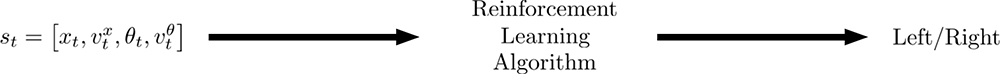
\includegraphics[scale=0.35]{Graphics/black_box_small.png}
% \caption[Reinforcement Learning Representation]{The black box is a representation of the reinforcement learning algorithm. The algorithm takes in a state from the environment, which passes through a black box to output the optimal action in the current state.}
% \label{fig:black_box}
% \end{figure}

Supervised machine learning approaches operate in distinct modes of training and inference. During training, an algorithm is shown labeled data and learns a representation of the underlying distribution of the data. After training, the model can be deployed to infer predictions based on the information it learns during training. However, supervised machine learning approaches are limited because they require labeled data, and labeled data is not always available. 

Reinforcement learning is a goal-oriented approach that is fundamentally different from supervised machine learning. The objective of reinforcement learning is to provide a means for an agent to continually learn while dynamically interacting with an environment. As the agent performs actions within the environment, it receives feedback through rewards and learns new behavior. The goal of the algorithm is to find the optimal actions at each given state. This is distinct from typical approaches in artificial intelligence, where an algorithm must first learn by viewing examples of a task being performed before it is capable of making predictions for this same task. 

However, there are many challenges to overcome in the field of reinforcement learning. First, reinforcement learning fails in area where it requires long-term strategy. Second, reinforcement learning requires a huge amount of training time and experience. Third, reinforcement learning is not robust to adjust to perturbations in the environment. This impediment is the main focus of this project. The goal is to investigate the sensitivity of reinforcement learning algorithms and try to develop a robust algorithm that can adapt to changes in the environment.

\section{Problem Statement}
This project focused on improving the flexibility of reinforcement learning algorithms, allowing them to adapt to perturbations in the environment. We explored common frameworks and algorithms in reinforcement learning and investigated techniques to reduce the power consumption and latency of the deployed model without compromising the accuracy of the system. We investigated the effects of enriching the feedback received by the agent to guide it towards more effective learning. Moreover, analysis of model efficiency revolved around characterizing the influence of hyperparameters and sensitivity to hardware devices.

%Reinforcement learning agents learn by exploring their environment 
%freely and receiving rewards for ideal behavior. A natural venue
%that provides such a sandbox is computer games. Computer games have well-defined environment, action, and reward. These games also do not require a physical device to interact with the environment. We can easily change the environment by varying the parameters of the game settings. Computer games fulfill the criteria for our exploration. We will particularly focus on a car racing game, which is potentially applicable to autonomous cars.

\section{Approach}
Computer games were used as a sandbox to explore the sensitivity of reinforcement learning algorithms. There are several advantages with using computer games: first, computer games have well-defined rules; second, they provide an efficient avenue for collecting data; third, the environment can be easily changed in order to induce perturbations. In particular, our investigations focused on an unsolved car racing challenge provided by the OpenAI Gym \cite{brockman2016openai}. The environment in the car racing game is interesting due to its application to autonomous cars. 

First, we implemented basic reinforcement learning algorithm with success in simple classic control games. Next, we implemented reinforcement learning algorithm incorporating deep learning, which produced promising results on a few classic control games and the Atari Breakout game. We then implemented deep Q-learning on the car racing game and explored the effect of reward clipping and regularization on performance. Lastly, we explored data compression in inputs to investigate how to reduce the storage required by the algorithm.

\section{Overview}
In this report, we will first explain the mathematical foundations of reinforcement learning in Chapter \ref{Ch:Reinforcement Learning}. Then we will focus on Q-learning and its implementation in Chapter \ref{Ch:Q-Learning-Representations}. We will present some of our successful results on some of the simple classic control and Atari games in Chapter \ref{Ch:ResultsPrelim}. We will discuss the results and findings while attempting to solve a car racing game in Chapter \ref{Ch:ResultsCarRacing} and \ref{Ch:Analyze}. Lastly, in Chapter \ref{Ch:FutureWork}, we provide ideas for future works needed to be done to make the algorithm more robust.

\endinput



% Chapter 2
\ifthenelse{\boolean{@twoside}}{\myclearpage}{}
\renewcommand{\S}{\mathcal{S}}
\newcommand{\A}{\mathcal{A}}
\newcommand{\R}{\mathcal{R}}
\newcommand{\M}{\mathcal{M}}
\renewcommand{\P}{\mathbb{P}}
\renewcommand{\E}{\mathbb{E}}

\chapter{Reinforcement Learning}\label{Ch:Reinforcement Learning}

In this chapter, we introduce the fundamental concepts of reinforcement learning algorithms. We start with a broad overview of reinforcement learning and dive into the basic principles of Markov Decision Processes, Value Functions, Bellman Optimality Equations and Temporal Difference Learning. 

\section{Reinforcement Learning Overview}\label{sec1}
\begin{figure}[h!]
\centering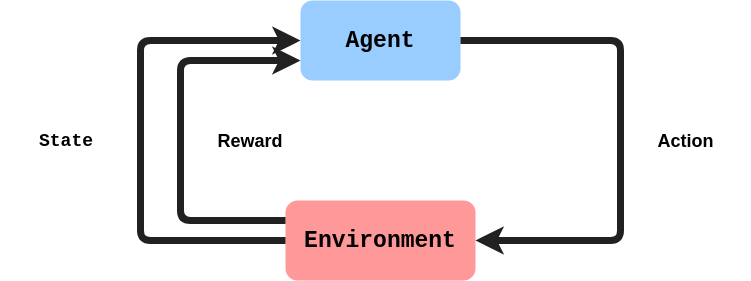
\includegraphics[scale=0.5,clip]{Graphics/RL_1.png}
\caption{Interaction of Agent and Environment}
\label{fig:RL_overview}
\end{figure}

Following \textit{Reinforcement Learning} by Sutton and Barto \cite{sutton1998reinforcement}, we define Reinforcement Learning as the field dedicated to the study of the Reinforcement Learning Problem (RLP). The Reinforcement Learning Problem can be defined broadly as the problem of learning from interaction to achieve a goal. The decision maker is called the \textit{agent}, while the world it interacts with is called the \textit{environment}. These two interact continually: the agent acts and the environment responds accordingly, presenting new situations to the agent. The environment also provides feedback to the agent via a scalar \textit{reward} signal. The goal of reinforcement learning is to learn a strategy, called \textit{policy}, that maximizes the expected cumulative reward the agent can receive. This process is illustrated in Figure \ref{fig:RL_overview}. In the following sections, we base our treatment of the material on \cite{szepesvari2010algorithms}. 

\section{Markov Decision Processes}\label{sec2}
The mathematical framework used to study the RLP, is the theory of Markov Decision Processes (MDPs), which allows for the modeling of sequential decision-making processes, subject to Markovian conditional independence assumptions. Here we restrict ourselves to countable MDPs, however there exist extensions to continuous state-action MDPs too. 

\begin{definition}
A Markov decision process is a tuple $ ( \S, \A, \P, \gamma) $ where
\begin{enumerate}
  \item $\S$ is a finite set of states
  \item $\A$ is a finite set of actions
  \item $\P := \P\left(S_{t+1} = \cdot, R_{t+1} = \cdot \mid S_t = \cdot,\ A_t = \cdot \right) : \S \times \mathbb{R} \times \S \times \A \rightarrow [0,1]$ is the state   transition probability matrix
  \item $\gamma \in [0,1]$ is the discount factor
\end{enumerate}
\end{definition}

Given an MDP $\M$, the interaction between the agent and its environment happens as follows: Let $t \in \mathbb{N}$ denote the current time, and let $S_t$ and $A_t$ denote the state of the environment and the action selected by the decisionmaker, respectively.  Upon receiving the action chosen by the agent, the environment makes a transition according to the dynamics of $\P$:
\begin{align}
  \left( S_{t+1}, R_{t+1} \right) \sim \P\left( S_{t+1} = \cdot, R_{t+1} = \cdot \mid S_t, A_t \right)
\end{align}

\begin{definition}
A policy $\pi \left( \cdot \mid \cdot \right) : \A \times \S \rightarrow [0,1]$ is a conditional probability distribution over actions, given the state. 
\end{definition}

Note that the policy fully defines the behavior of the agent. The last notion we need to define the problem is the \textit{return}.

\begin{definition}
The return underlying a policy $\pi$ is defined as the total discounted sum of the rewards incurred:
\begin{align}
  \R = \sum\limits_{t=0}^{\infty} \gamma^{t} R_{t+1}
\end{align}
\end{definition}

The goal of the agent is to learn a policy that performs well. Our measure of performance is the \textit{expected return}--a rather natural metric. 

\section{Value Functions}\label{sec3}
Given the expected return characterization of performance, we can compare two policies and decide which one leads to better rewards. But how do we find good policies? The optimal value $V^* (s)$ of $s \in \S$ is the highest achievable expected return when the process is started from state $s$. We call $V^*:\S \rightarrow \mathbb{R}$ the optimal value function, and if a policy $\pi_*$ achieves these optimal values in all states, it is called an \textit{optimal policy}. We can extend the notion of value function to arbitrary policies: 

\begin{definition} The value function $V^{\pi} : \S \rightarrow \mathbb{R}$ underlying the policy $\pi$ is defined as
\begin{align}
  V^{\pi} \left( s \right) = \E \left[ \R \mid S_0 = s \right] = \E \left[\sum\limits_{t=0}^{\infty} \gamma^{t} R_{t+1} \mid S_0 = s \right]
\end{align}
where the values $R_{t+1}$ are obtained following policy $\pi$. 
\end{definition}

A related object is the action-value function of a policy $\pi$. 

\begin{definition} The action-value function $Q^{\pi} : \S \times \A \rightarrow \mathbb{R}$ underlying the policy $\pi$ is defined as
\begin{align}
  Q^{\pi} \left( s, a \right) = \E \left[ \R \mid S_0 = s, A_0 = a \right] = \E \left[\sum\limits_{t=0}^{\infty} \gamma^{t} R_{t+1} \mid S_0 = s, A_0 = a \right]
\end{align}
where the values $R_{t+1}$ are obtained following policy $\pi$. 
\end{definition}

Similar to the way we defined $V^*$, we can define the optimal action-value function $Q^*$, given to rise by the optimal policy $\pi_*$. Due to the Markov property, given $V^*$ and $\P$, we can easily devise an optimal policy: in a given state, choose the action that leads to maximal average $V^*$ value. With Q we can do even better: Given just $Q^*$, the policy $\pi(s) = \arg\max\limits_{a \in \A} Q^*(s, a)$ is optimal. Note that in the MDPs considered here, an optimal policy always exists. 

\section{Bellman Optimality Equations}\label{sec4}
Denote $r(s,a) := \E \left[ R_{t+1} \mid S_t = s,\ A_t = a \right]$. Then the optimal value function $V^*$ and $Q^*$ are connected by the following equations: 
\begin{align}
V^* (s) &= \sup\limits_{a \in \A} Q^* (s, a) \label{eq:V-opt-simple} \\
Q^* (s, a) &= r(s,a) + \gamma\ \E\left.\left[ V^* \right| S_t=s,\ A_t=a \right] \label{eq:Q-opt-simple} \\
&=  r(s,a) + \gamma\ \sum\limits_{w \in \S} \P \left( S_{t+1}=w \mid S_t = s,\ A_t = a \right) V^*(w)\\
\end{align}

These can be shown to hold by simple conditioning arguments. Intuitively they can be thought of as saying the following: Suppose we are following an optimal policy $\pi_*$. By optimality, in state $s$, we must choose an action with maximal state-action value $Q^*$. But then it must be that $V^*$ is equal to this maximal value, and Equation (\ref{eq:V-opt-simple}) follows. Equation (\ref{eq:Q-opt-simple}) follows by a similar argument. Combining these two equations gives rise to the Bellman Optimality Equations: 
\begin{align}
V^* (s) &= \sup\limits_{a \in \A} \left\lbrace  r(s,a) + \gamma\ \sum\limits_{w \in \S} \P \left( S_{t+1}=w \mid S_t = s,\ A_t = a \right) V^*(w) \right\rbrace \label{eq:V-opt} \\
Q^* (s, a) &=  r(s,a) + \gamma\ \sum\limits_{w \in \S} \P \left( S_{t+1}=w \mid S_t = s,\ A_t = a \right) \sup\limits_{a \in \A} Q^* (w, a) \label{eq:Q-opt}
\end{align}

A short proof of Equation (\ref{eq:Q-opt}) is given in the next section. Introducing new notation, we can rewrite Equation (\ref{eq:V-opt}) more succinctly, in a way that suggests a solution:

\begin{definition}
Define the Bellman Optimality operator $T^*: \mathbb{R}^\S \rightarrow \mathbb{R}^\S $, by
\begin{align}
(T^*V)(s) = \sup\limits_{a \in \A} \left\lbrace  r(s,a) + \gamma\ \sum\limits_{w \in \S} \P \left( S_{t+1}=w \mid S_t = s,\ A_t = a \right) V(w) \right\rbrace
\end{align}
Then the Bellman Optimality Equation for V can be rewritten as 
\[
T^*V^* = V^*
\]
\end{definition}

An analogous operator exists for $Q^*$ that we don't cover here. Under certain conditions, it can be shown that both (nonlinear) Bellman Optimality operators are in fact contractions. Thus, by a fixed point argument, they have unique solutions that can be iteratively approximated. Such iterative approximations have been the bases of many of the early reinforcement learning algorithms. 

\section{Temporal Difference Learning}\label{sec5}
Instead of pursuing these fixed point approximation methods, we turn to the more sophisticated Temporal Difference (TD) Learning approach, one of the most significant ideas in reinforcement learning. Recall the optimality equation for $Q^*$:
\begin{align}
Q^*(s_t, a_t) &= \E\left.\left[R_{t+1} + \gamma R_{t+2} +
\gamma^2 R_{t+3} + \cdots = \sum_{i=t}^{\infty} \gamma^{i-t}R_{i+1}
\right| S = s_t, A = a_t \right] \\
&= \E\left.\left[R_{t+1} + \E\left.\left[ \sum_{i=t + 1}^{\infty} \gamma^{i-t}R_{i+1}
\right| s_t, a_t, S_{t+1} \right] \right| S = s_t, A = a_t \right] \nonumber \\
&\stackrel{*}{=} \E\left.\left[R_{t+1} + \gamma\ \max\limits_{a' \in \A} \E\left.\left[ \sum_{i=t + 1}^{\infty} \gamma^{i-(t + 1)}R_{i+2}
\right| S_{t+1}, A_{t+1}=a' \right] \right| S = s_t, A = a_t \right] \nonumber \\
&= \E\left.\left[R_{t+1} + \gamma\ \max\limits_{a' \in \A} Q^*(S_{t+1},a') \right| S = s_t, A = a_t \right] \label{eq:Q-optimality}
\end{align}

where the starred equality follows by the Markov property and the fact that we follow the optimal policy $\pi_*$. This splits $Q^*$ into two quantities: the immediate reward and the discounted
future rewards. More importantly,
Equation (\ref{eq:Q-optimality}) reveals structure that 
immediately yields a suitable iterative update shown in Equation (\ref{eq:q_iter_up}).
\begin{align}\label{eq:q_iter_up}
Q(s_t, a_t)_{j+1} &= Q(s_t, a_t)_j + \alpha \;
\left(R_{t+1} + \gamma \; \underset{a'}\max \; Q(s_{t+1},a') - Q(s_t, a_t)\right)
\end{align}
where $\alpha \in [0, 1]$. As $\alpha$ approaches 1, 
the $Q$ value function is constructed to weight the 
future rewards more heavily. 

This update is in the standard iterative update format
$Q(s_t, a_t)_{j+1} = Q(s_t, a_t)_j + \alpha \times \textrm{error} $ where
the error captures the difference between what the value $Q(s_t, a_t)$ 
\textit{should} 
be at the current iteration: $R_{t+1} + \gamma \; \underset{a' \in \A}\max \; Q(s_{t+1},a')$ 
and what it is at the current iteration: $Q(s_t, a_t)$. 

In the next section we expand on this idea, and introduce the Q-learning algorithm, which will form the basis of our investigations. 
\endinput




% Chapter 3
\ifthenelse{\boolean{@twoside}}{\myclearpage}{}
\chapter{Q-Learning}\label{Ch:Q-Learning-Representations}

The previous chapter presented the backbone of Q-learning. In this chapter, we explain the details for implementing Q-learning algorithms. In section \ref{tabQ}, we demonstrate a tabular approach with the Cart Pole game as an example. The detailed results will appear in Chapter \ref{Ch:ResultsPrelim}. In section \ref{deepQ}, we explain the theoretical background for deep Q-learning. We introduce regularization in section \ref{reg}, which is the technique we used to improve our results in Chapter \ref{Ch:Analyze}.

\section{Tabular Q-Learning}\label{tabQ}
Having established the theoretical aspects of $Q$, it is necessary to find a 
suitable representation that can be found computationally. Two such 
representations will be discussed; here, a tabular representation is
described.

In the tabular setting, $Q$ will be represented by a look-up table where every
row corresponds to a state of the game and the respective columns represent
actions. Due to finite computational memory, storing the value of $Q$ for 
every possible state-action pair is infeasible when state spaces are continuous.
Consequently, continuous parameters from state spaces must be discretized into
disjoint bins. An example of such a discretization is given in Table 
\ref{table:disc_state_ex} for the game of Cart Pole.

\begin{table}[h!]
\centering
$\begin{aligned}[t]
x_t \in [-2.4, 2.4] &\Rightarrow {\{[-2.4, -0.8), [-0.8, 0.8), [0.8, 2.4]\}} \\
v_t^x \in [-\infty, \infty] &\Rightarrow {\{[-2, -1), [-1, 0),[0,1), [1, 2]\}}  \\
\theta_t \in [-0.419, 0.419] &\Rightarrow {\{[-0.419, -0.14), [-0.14, 0.14), [0.14, 0.419]\}}  \\
v_t^{\theta} \in [-\infty, \infty] &\Rightarrow {\{[-2, -1), [-1, 0), [0, 1), [1,2]\}} \\
\end{aligned}$
\caption[Discretized state space]{Since the state space is continuous, in order to represent the $Q$ function as a table, it is critical to discretize the state space.}
\label{table:disc_state_ex}
\end{table}

Once the state space has been discretized, each state can be mapped to its
corresponding bin which can then be mapped to a row in the tabular representation
of $Q$. An example of $Q$ for Cart Pole at some iteration is given in 
Table \ref{table: tab_q_ex}.

\begin{table}[h!]
\centering
\begin{tabular}{ c|c|c } 
  & Left & Right \\
 \hline
 {[1, 1, 1, 1]} & 0.8 & 0.3 \\
 {[1, 1, 1, 2]} &  & 0.6 \\
 \vdots & \vdots & \vdots \\
 {[2, 1, 2, 3]} & 0.15 & 0.11 \\
 \vdots & \vdots & \vdots \\
 {[3, 4, 3, 4]} & 1.2 & 0.9 \\
\end{tabular}
\caption[Tabular $Q$ example]{This table is an example of how to represent $Q$ function as a table. This table in particular stores the $Q$ function for the game Cart Pole, which was solved by the team. The details about solving Cart Pole is in Chapter \ref{Ch:ResultsPrelim}}
\label{table: tab_q_ex}
\end{table}

\subsection{Drawbacks}
While the tabular representation of $Q$ is favorable for pedagogical purposes and 
its implementation ease, it does not generalize well to games with large state 
spaces. For example, a gray-scale image with 1000 pixels has a state space size 
of $256^{1000}$. Storing values for each state is noticeably infeasible. Rather 
than storing the value of $Q$ for every possible state, we will use a function
to approximate $Q$. In particular, we will use a neural network to approximate
$Q$, as discussed in the next section.

\section{Deep Q-Learning}\label{deepQ}
\subsection{Overview}
In this section we outline the Deep Q-Learning (DQN) algorithm, which we took as the starting point 
of our investigation into Deep Reinforcement Learning. The basic idea of DQN is to represent the 
state-action value function Q as a convolutional neural network--recent work has shown deep neural networks to work
well in this setting. 

There are three simple modifications one has to make to the tabular Q-Learning algorithm to get what 
is now commonly called the DQN-algorithm \cite{mnih2013playing}. We outline these modifications below. 

\subsection{Q as a neural network}
The first step is to replace the function $Q:S\times A \rightarrow \mathbb{R}$ by a neural network \linebreak
${Q(\cdot, \cdot \mid \theta):S \times A \rightarrow \mathbb{R}}$, where $\theta$ denotes the weights of the model.
The resulting network, called 
the Q-network, takes as its input a state and an action, and outputs the estimated Q-value of the 
pair. But the question arises: How do we find good parameters $\theta$ for this model? Suppose that
 at timestep $i$ we have current estimates $\theta_i$ for the weights of the network. We take the loss function to be the mean squared TD-error, the same error term as used in the simple 
 tabular Q-learning algorithm, derived from the Bellman optimality equation. 
\begin{align}
L_i(\theta_i) = \mathbb{E} \left[ \left( \E\left.\left[ R_{t+1} + \gamma\, \max\limits_{a'} Q(s_{t+1}, a' \mid \theta_{i-1}) \right| s_t, a_t \right] - Q(s_t, a_t \mid \theta_i) \right)^2 \right]
\end{align}

Because the dynamics of the environment the agent is operating in is unknown, the expectation above cannot be evaluated;
we get around this by using Stochastic
Gradient Descent (SGD). Using this method,
we get the following update rule for the weights $\theta$ :
\begin{align}
\nabla_{\theta_i} L_i (\theta_i) &= \mathbb{E} \left[ \left(R_{t+1} + \gamma\, \max\limits_{a'} Q(s_{t+1}, a' \mid \theta_{i-1}) - Q(s_t, a_t \mid \theta_i) \right) \nabla_{\theta_i} Q(s_t, a_t \mid \theta_i ) \right] \\
\theta_{i+1} &= \theta_i - \alpha\, \nabla_{\theta_i} L_i (\theta_i) \rvert _{\theta_i}
\end{align}

\subsection{Experience Replay and Fixed Q-Targets}
In theory, SGD only works under some independence assumptions on the data 
we feed it. We need to ask ourselves whether these assumptions are reasonable in this setting. As 
we are playing the game, and updating our weights at each timestep, the sequence of transitions 
visited by the agent is highly correlated: We cannot reasonably expect the game's state to be independent
of its immediate past. Therefore, we use the method of experience replay to decorrelate the data and  
to achieve higher data efficiency. Moreover, this helps 
reduce the risk of getting stuck  in unwanted feedback loops. 

At each timestep, we store the tuple $(s_t, a_t, R_{t+1}, s_{t+1})$ in the replay memory denoted by 
$\mathcal{D}$. Instead of updating $\theta$ based on the most recent transition, we instead sample 
uniformly from $\mathcal{D}$, and use these past experiences to perform the gradient descent step. 
In practice, we sample a minibatch of transitions $(s_j, a_j, R_{j+1}, s_{j+1})_{j \in J}$ where the 
minibatch size $|J|$ is usually chosen to be a multiple of 2 in the range of 16 to 64. This way we reuse all experiences
 multiple times during training. Another parameter that arises from experience replay is the replay 
 memory capacity - the maximum length of the replay memory - which is chosen in the range of $10^3$ to $10^6$.

The final modification that needs to be made in order for DQN to work is the method of fixed Q-targets. 
In the loss function, in the absence of supervision, one must bootstrap from the current weights $\theta_i$ 
in order to arrive at the TD-error, an estimate of Q's accuracy. However, instead of using the most recent 
estimates $\theta_i$, one can use a separate, periodically updated set of weights, usually denoted by $\theta^-$. 
After the modification, the loss function becomes 
\begin{align}
L_i(\theta) = \mathbb{E} \left[ \left( \E\left.\left[ R_{t+1} + \gamma\, \max\limits_{a'} Q(s_{t+1}, a' \mid {\color{red} \theta^-}) \right| s_t, a_t \right] - Q(s_t, a_t \mid \theta) \right)^2 \right]
\end{align}

\begin{figure}[h!]
\centering\includegraphics[scale=0.25,clip]{Graphics/ipam.png}
\caption[Downsampling and Flattening the Logo of IPAM]{This is an illustration of the pre-processing method commonly employed in RL algorithms.}
\label{fig:ipam}
\end{figure}

\newpage
\section{Q-learning in practice}
We now address the question of how the data used to train
the agent is generated. In practice, $Q$ is initialized randomly, thus immediately taking the actions suggested
by $Q$ as in Equation (\ref{eq:q_iter_up}) will introduce bias towards the 
initialization of $Q$. As such, the agent is expected to explore the state space 
and determine which actions are more suitable for certain states. Consequently,
a parameter $\epsilon \in [0,1]$ will be used to determine which action to take
at each iteration: with probability $\epsilon$, a random action will be taken; 
with probability $1 - \epsilon$ the action suggested by $Q$ will be taken. In more complex computer games, the only observation the agent is given 
by its environment is an RGB image of the screen for each frame of the game. We process these images, 
in order to be able to use them as input to the Q-network. We do so following the methods used by Mnih et al. in \textit{Playing Atari with Deep Reinforcement Learning} \cite{mnih2013playing}:
at each timestep, we take the most recent four frames, convert them to grayscale, downsample to a size 
of $84\times 84$, and then stack them to produce the input to the network. A toy visualization of this process is given in
Figure \ref{fig:ipam}.

\section{Regularization}\label{reg}
A common problem among machine learning algorithms is 
that the algorithm often overfits to the training data 
and struggles to generalize to new inputs during testing. 
Many strategies have been developed to address this, possibly at the expense of increasing the training 
error. These strategies are collectively called regularization. 
\par
In deep learning, most regularization strategies are based on 
regularizing estimators, such as parameter norm penalties where 
parameters are penalized based on its norm. In other words, the 
larger the effect a parameter has on the outcome, the more heavily 
the parameter will be penalized, forcing the algorithm to not 
overfit to certain features during training. 
\par
In our project, we chose \textbf{dropout} as our regularization method as
it provides a computationally inexpensive method for 
regularizing the models. The next section expands on the
theoretical aspects of dropout.

\subsection{Dropout}
Dropout was first introduced by Srivastava et al. in 2014 
\cite{JMLR:v15:srivastava14a} as a regularization method. Dropout 
drops units (along with their connections) from the neural 
network during training, preventing estimators from 
co-adapting to the training samples. Alternatively, dropout can be understood in the context of bagging. In particular, dropout separates a large neural network
into an ensemble of of many sub-networks, which is similar to bagging. Bagging involves training multiple models and evaluating multiple models for each test case. However, bagging becomes impractical when it comes to large neural networks due to the huge amount of training time and computational power required. Dropout provides a way to implement bagging on large neural networks since it essentially trains sub-networks at once and infers the results from the collective knowledge of all sub-networks.

\begin{figure}[h!]
\centering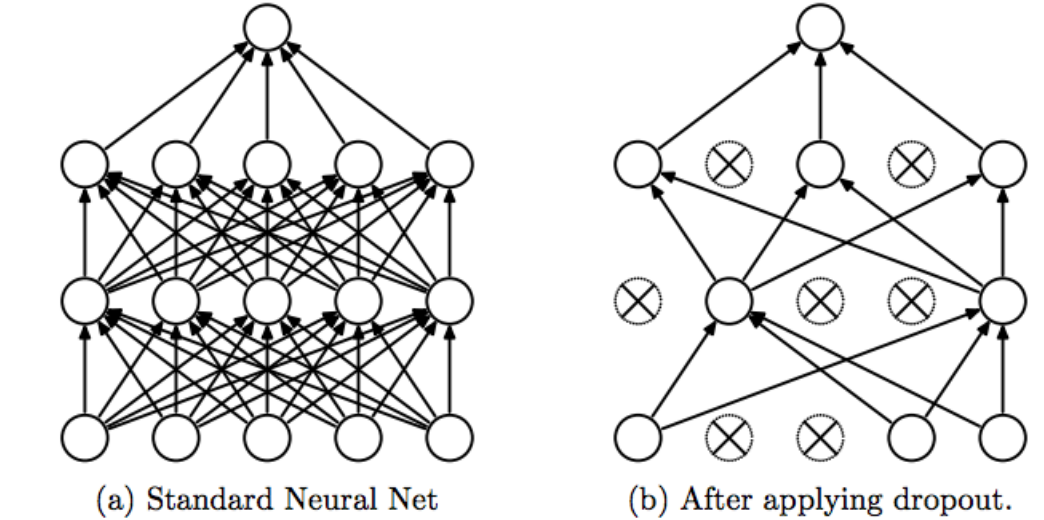
\includegraphics[scale=0.3,clip]{Graphics/dropout.png}
\caption[Illustration of Dropout]{This figure shows how dropout decomposes a connect neural network into sub-networks. The cross marks on neurons indicate that the neurons are zeroed out and not included in the sub-network.}
\label{fig:dropout}
\end{figure}

Dropout seeks to divide a large neural network into sub-networks by `dropping out' some of the neurons in the network. During training, a mask containing zeros and ones is randomly generated based on a hyperparameter for determining the percentage of neurons to keep in the sub-networks. This mask is then applied to the neural network, zeroing the weights of some neurons. By performing this operation, a large neural network is decomposed into sub-networks. During inference, the result is calculated based on the geometric mean of the results from all sub-models given by
\begin{align}
\tilde{p}_{ensemble}(y | \boldsymbol{x})=\sqrt[2^d]{\prod_{\boldsymbol{\mu}} p(y | \boldsymbol{x},\boldsymbol{\mu})}
\end{align}

where $\boldsymbol{\mu}$ is the randomly generated mask, d is the number of neurons that may be dropped, $\boldsymbol{x}$ is the input and $y$ is the predicted output.
\par
After taking the geometric mean, it is necessary to normalize the ensemble:
\begin{align}
p_{ensemble}(y | \boldsymbol{x})=\frac{\tilde{p}_{ensemble}(y | \boldsymbol{x})}{\sum_{y'} \tilde{p}_{ensemble}(y' | \boldsymbol{x})}
\end{align}

Dropout is a commonly used regularization method in deep neural networks. It is commonly believed that dropout is not necessary for deep RL algorithms because overfitting does not occur often in the RL realm. Due to the large state space, it is not likely for the model to overfit to the environment. However, we provide an counter example in Chapter \ref{Ch:Analyze} to demonstrate that the use of dropout could improve performance and save training time by generalizing model trained in a fixed environment.


\endinput



% Chapter 4
\ifthenelse{\boolean{@twoside}}{\myclearpage}{}
\chapter{Preliminary Results}\label{Ch:ResultsPrelim}

In this chapter, we briefly discuss the preliminary results we obtained on simpler games. In section \ref{sec:tabQ}, we present our successes with implementing tabular Q-learning on classic control games, Cart Pole and Mountain Car. We then show our results using deep Q-learning on a Atari game, Breakout, in section \ref{sec:deepQ}.

\section{Tabular Q-Learning Results}\label{sec:tabQ}

\begin{figure}[h!]
\centering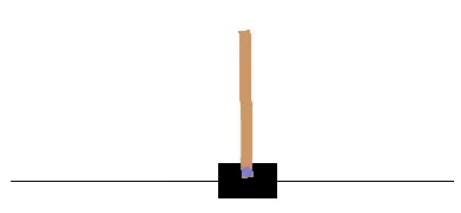
\includegraphics[scale=0.45,clip]{Graphics/cartpole.png}
\caption[Cart Pole]{The game environment of a simple classic control game, Cart Pole}
\label{fig:cartpole}
\end{figure}

We initially investigated two simple games from the OpenAI Gym toolkit. The first game was Cart Pole, where the goal is to balance a pole in a cart for as long as possible. In this game, the state is represented as a four-dimensional vector containing the values for the position of the cart, the velocity of the cart, the angle of the pole, and the velocity of the pole. The game is considered solved when the agent achieves an average score $\geq$ 195 over 100 consecutive trials. Using the tabular Q-learning approach, the algorithm achieved a perfect score of 200 over 100 consecutive trials. This score was achieved with a bucket size of 1 for the position and velocity of the cart and a bucket size of 20 for the angle and velocity of the pole for state space discretization. This agent was trained for 500 episodes with a discount factor of 0.99, minimum learning rate of 0.05, and minimum explore rate of 0.1.

\begin{figure}[h!]
\centering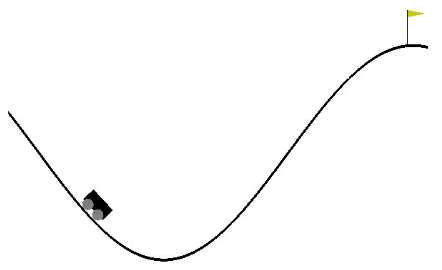
\includegraphics[scale=0.45,clip]{Graphics/mountain_car.png}
\caption[Mountain Car]{The game environment of a simple classic control game, Mountain Car}
\label{fig:mountain_car}
\end{figure}

We also trained the tabular Q-learning algorithm for the Mountain Car game. In this game, the goal is for the car to reach the top of the mountain as quickly as possible. We initially faced challenges with this game due to the nature of the reward function. Since the reward function returns a negative reward for each time step, it is difficult to reinforce positive behavior before actually winning the game. As a result, the performance varied as a result of slight changes in parameters. After experimentation, the algorithm performed best with a bucket size of 10 for position, bucket size 30 for velocity, discount factor of 0.99, fixed learning rate of 0.05 and fixed explore rate of 0.1. After training for 10,000 episodes, the algorithm achieved an average reward of -157.64 over 100 test episodes.

\section{Deep Q-Learning Results}\label{sec:deepQ}
Next, we implemented the Deep Q-Learning algorithm on the Atari Breakout and Pong games using the convolutional architecture as defined in \cite{mnih2013playing}. The first layer of the neural network was a convolutional layer with 32 kernels, 8x8 filter, and stride 4x4. The second was a convolutional layer with 16 kernels, 4x4 filter, and stride 2x2. The third layer was a dense layer with 256 neurons and a nonlinear rectifier. The final layer was a dense layer with 16 neurons and a linear rectifier. The performance was quantitatively analyzed using average Q-values. Assuming that $S$ is a uniform sample of $n$ fixed states, an estimate of the average Q-value was computed as follows.
$$ Q_{avg} = \frac{1}{n} \sum_{i=1}^{n} max_{a} Q(s_{i},a) ~~~ s_{i} \in S$$

Using this architecture, the algorithm was able to achieve promising results on both Breakout and Atari with the former shown in \ref{fig:breakout}. The average Q-value appeared to increase over time and eventually converge, essentially recreating the results described in \cite{mnih2013playing}.

\begin{figure}[h!]
\centering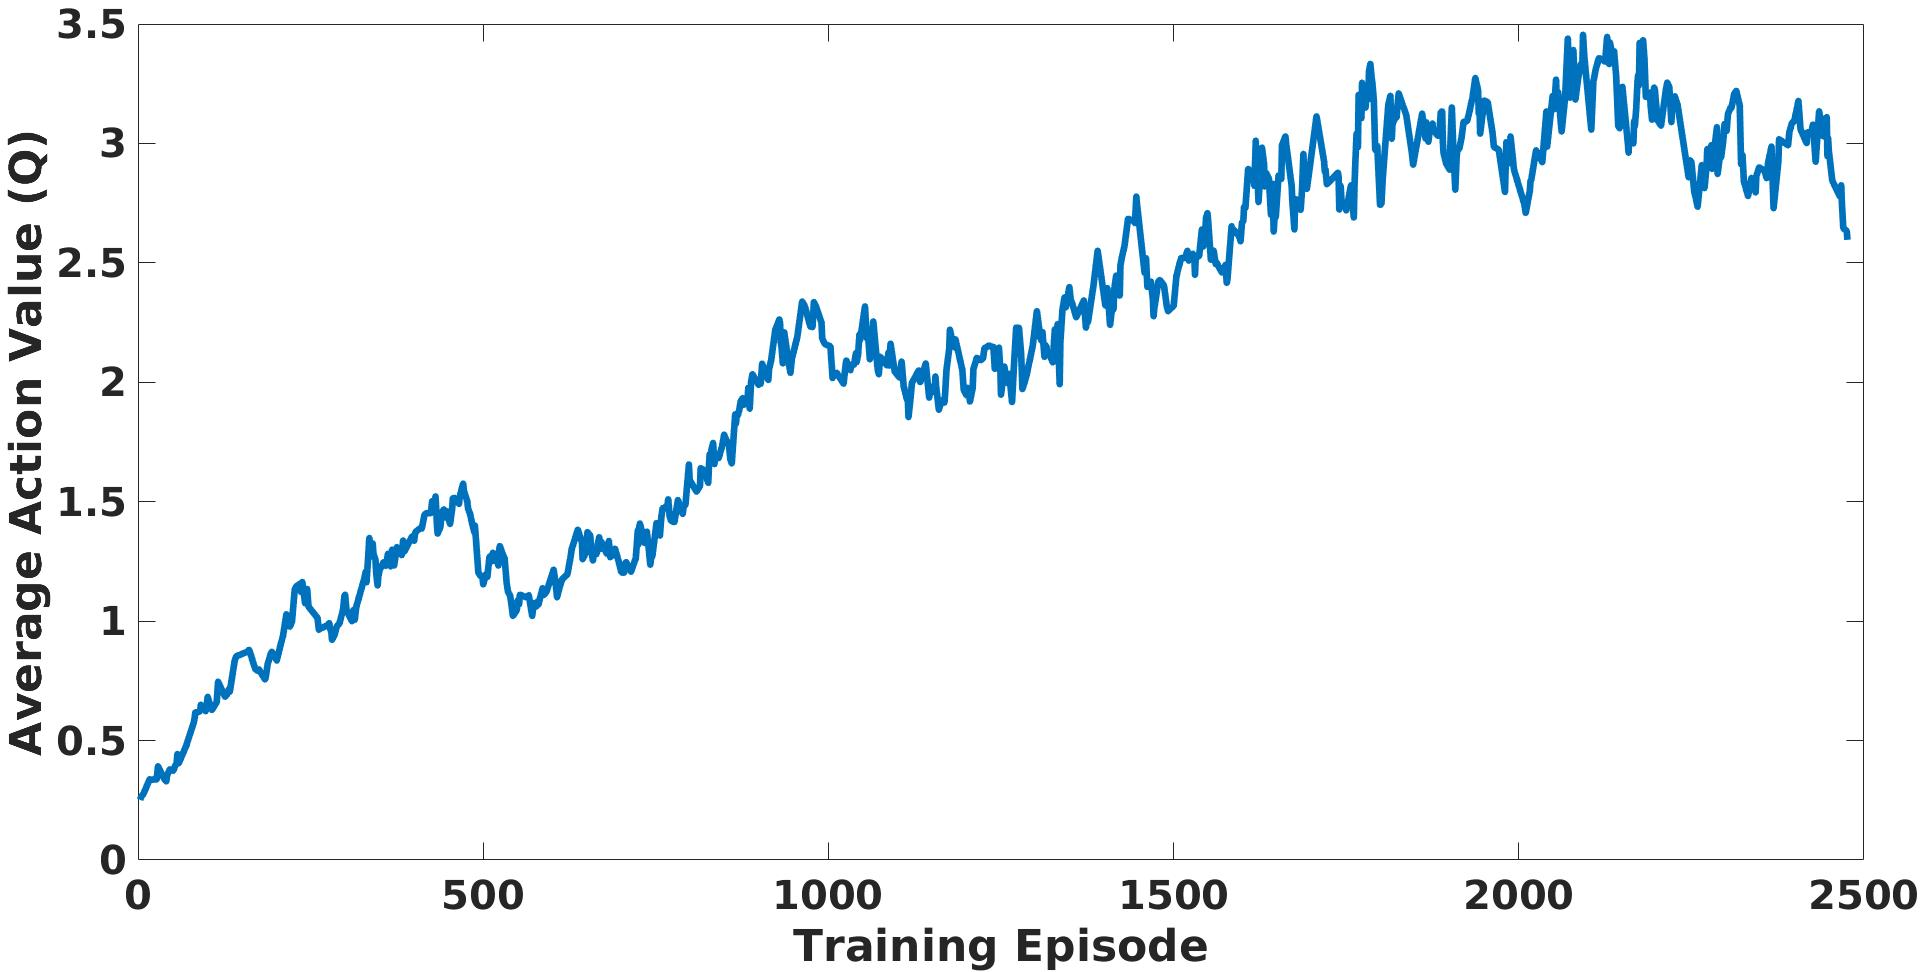
\includegraphics[width=0.6\textwidth]{Graphics/breakout_AveQ.jpg}
\caption[Average Action Value Plot for Breakout]{Average action value converges as expected}
\label{fig:breakout}
\end{figure}

\endinput





% Chapter 5
\ifthenelse{\boolean{@twoside}}{\myclearpage}{}
\chapter{Autonomous Driving}\label{Ch:ResultsCarRacing}

After verifying the correctness of our implementation by applying it
to simpler environments such as Cart Pole and Breakout, we moved on to
working on OpenAI's CarRacing environment, which is a 2-dimensional
car racing game. In section \ref{sec1}, we go over the CarRacing
environment in detail. We explore the effect of neural network
structure, action space and reward feedback in the following sections.  

\section{The OpenAI CarRacing Environment}\label{sec1}
\begin{figure}[h!]
\centering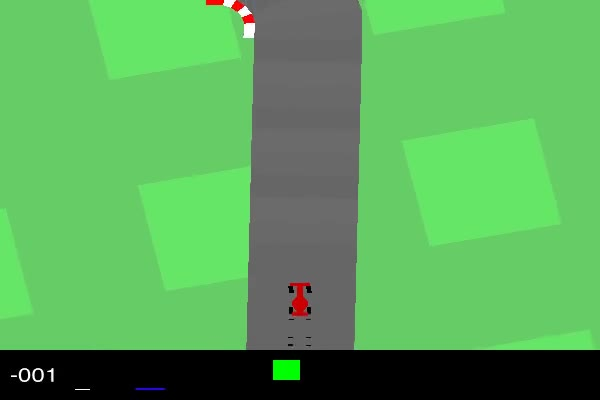
\includegraphics[scale=0.45,clip]{Graphics/carracing.jpg}
\caption[Car Racing]{The game environment of the car racing game}
\label{fig:carracing}
\end{figure}
In OpenAI's CarRacing environment - from here on referred to as the
`car racing game' - the emulator provides 96 by 96 RGB screenshots to
the agent, which has control over a red racing car, as shown in Figure
\ref{fig:carracing}. Notice that the track is made up of distinct
tiles. The reward signal is -0.1 for every frame passed and
$\frac{1000}{N}$ for every tile visited, where N is the total number
of tiles on the track. Thus the goal of the game is to finish the
track as fast as possible, without missing any of the tiles. The
actions come in the form of an array of three numbers. In the array,
the first number indicates steer, the second number indicates
acceleration and the third number indicates deceleration. The steer
coordinate is continuous from -1 to 1 while the acceleration and the
deceleration are continuous from 0 to 1. For example, if the agent
finishes in 732 frames and never leaves the track doing so, the reward
is 1000 - 0.1*732 = 926.8 points. The episode finishes when all tiles
are visited or more than 1000 frames pass. As per OpenAI's guidelines,
the environment is solved when an average score of 900 or more is
achieved over 100 episodes.  
\par
We chose this environment for several reasons: first, the car racing
game is similar to real life autonomous driving; second, the game
environment can be easily altered, allowing for interesting
exploration of robustness of Deep RL methods; third, according to the
leaderboard on OpenAI's website, no one has successfully solved the
game.  
\par
To be able to iterate faster, we created four different types of
training environment of varying complexity: random short tracks, fixed
one track, fixed three tracks and random tracks. In the random short
track environment, there are 50 tiles for the agent to finish while in
the other environments, there are approximately 300 tiles. Random
short tracks and random tracks environment display randomly generated
tracks for each episode while the other environments display the same
one (fixed one track) or three tracks (fixed three tracks). 

\section{Network Architecture}
When we first started working on the car racing environment, the 2
convolutional layer architecture used in Chapter 4 and
\cite{mnih2013playing} was used. However, considering the complexity
of the game, a deeper three-convolutional architecture was tested. 

\begin{figure}[h]
\centering
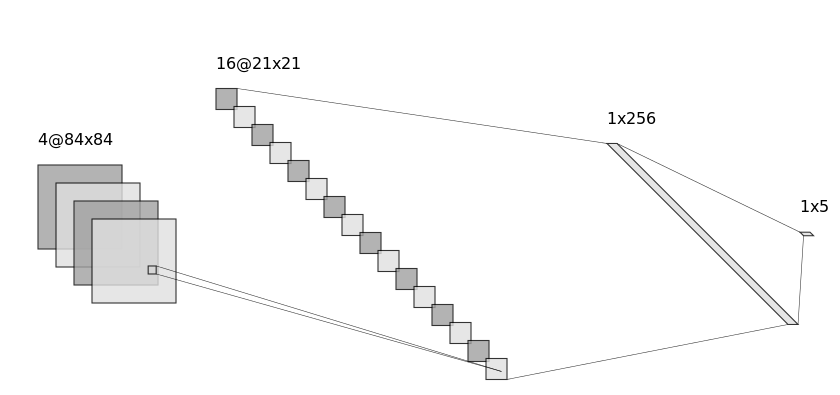
\includegraphics[width=0.6\textwidth]{Graphics/nn_crop2.png} 
\caption[Two Convolutional Neural Network Structure]{Neural Network
  with two convolutional layers. Specific parameters are in Table
  \ref{table: neuralstructures}.} 
\label{fig:2conv}
\end{figure}

\begin{figure}[h]
\centering
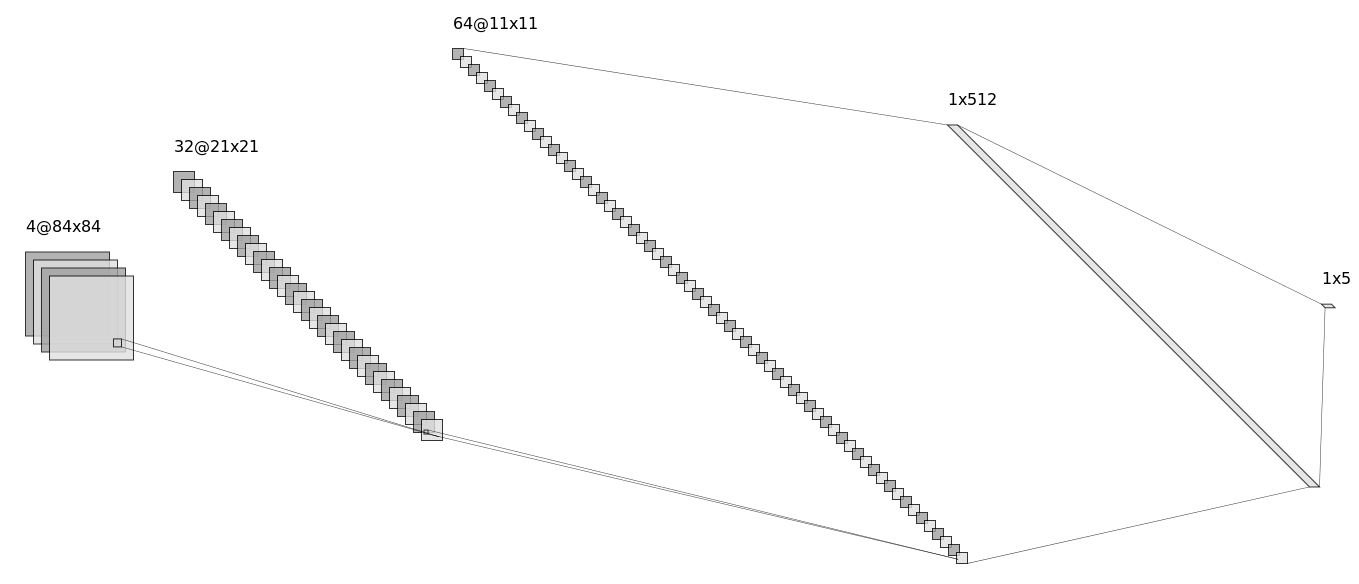
\includegraphics[width=0.6\textwidth]{Graphics/nn_crop3.png}
\caption[Three Convolutional Neural Network Structure]{Neural Network
  with three convolutional layers. Specific parameters are in Table
  \ref{table: neuralstructures}.} 
\label{fig:3conv}
\end{figure}

We trained these two neural network structures in the random short
tracks environment.  

\begin{figure}[h]
\centering
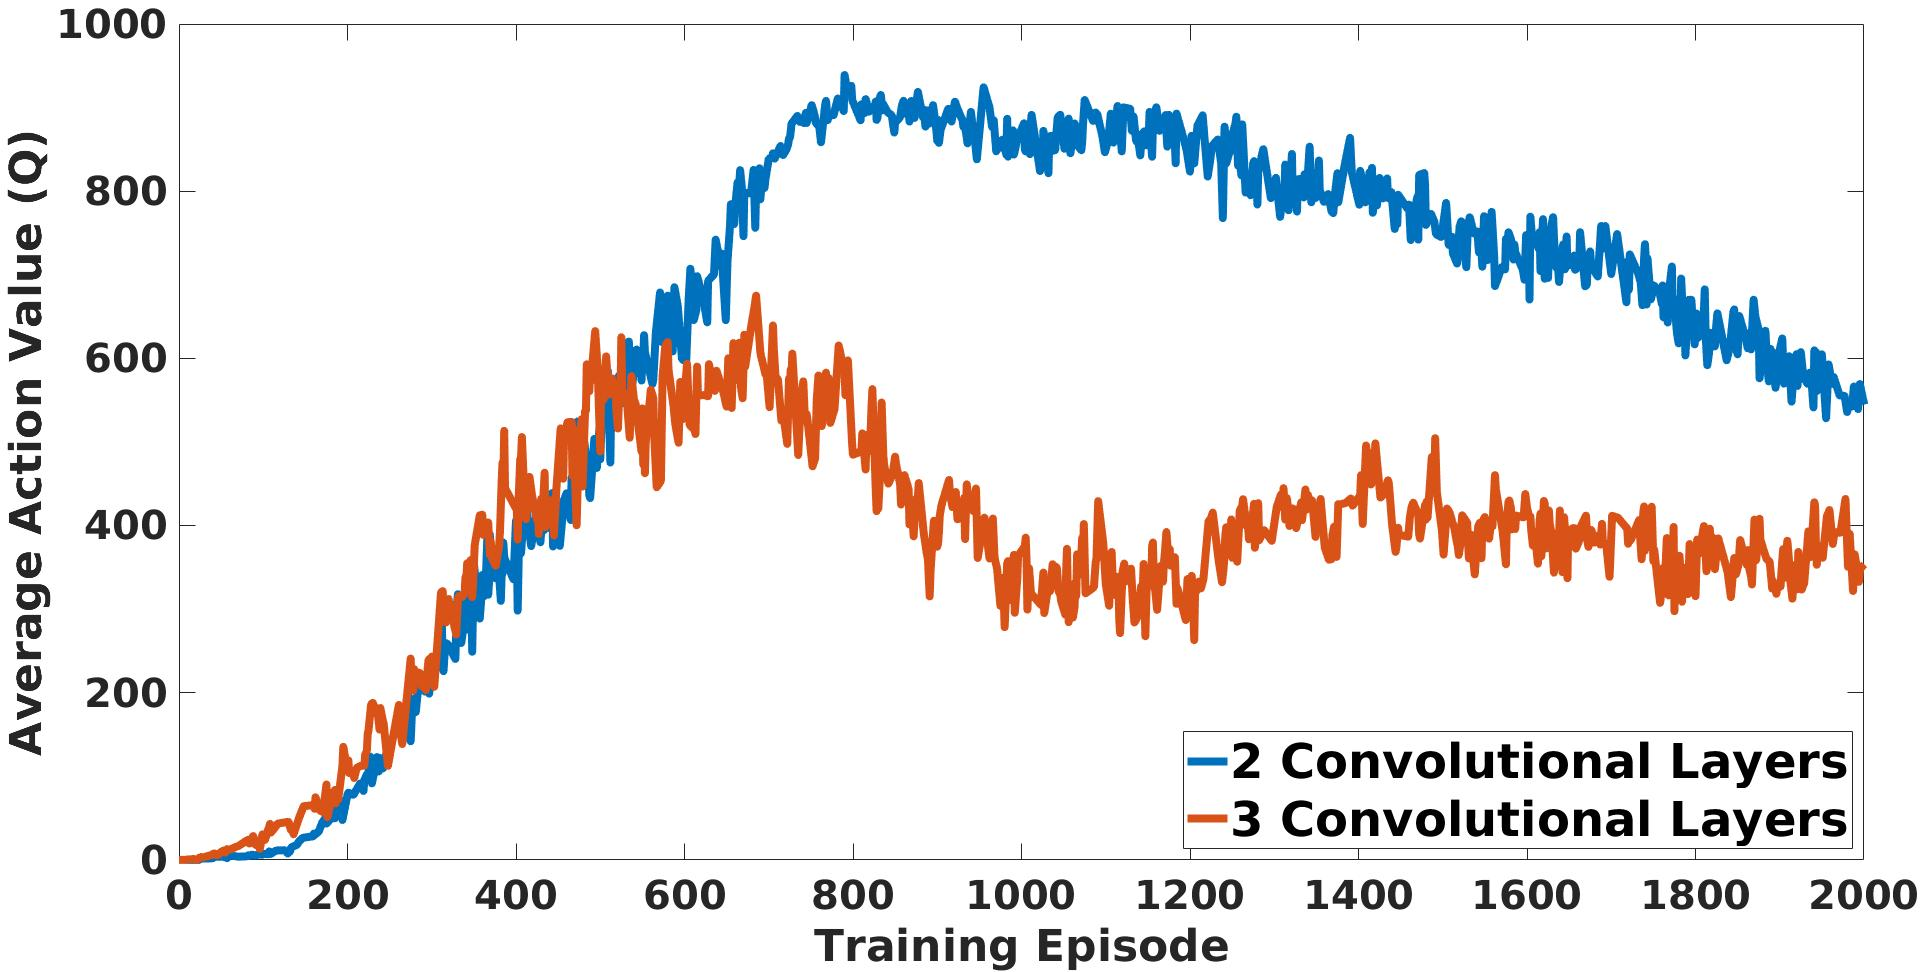
\includegraphics[width=0.6\textwidth]{Graphics/AveQ_conv.jpg}
\caption[Average Action Values Neural Network Structure
  Comparison]{Average action values using two convolutional layers
  (orange) and three layers (blue).} 
\label{fig:conv_aveq}
\end{figure}

\begin{figure}[h]
\centering
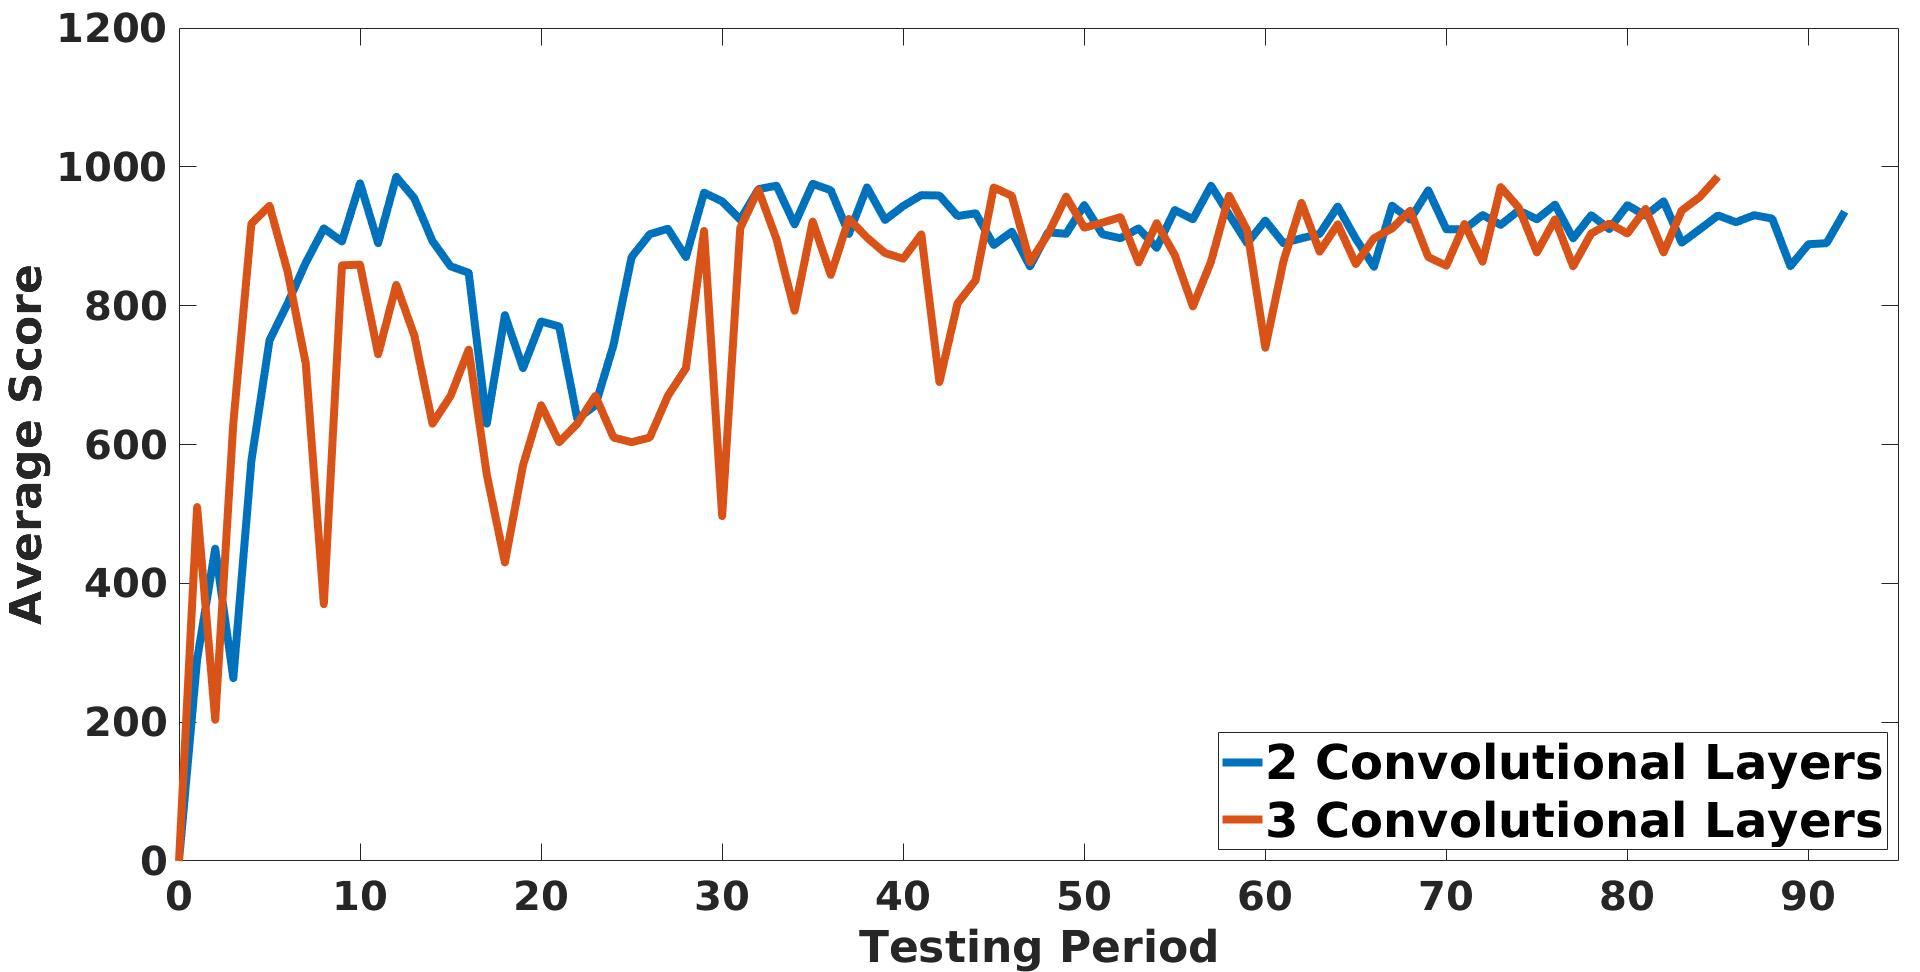
\includegraphics[width=0.6\textwidth]{Graphics/TestScore_conv.jpg}
\caption[Average Test Score Neural Network Structure
  Comparison]{Average score over five tests using two convolutional
  layers (orange) and three layers (blue).} 
\label{fig:conv_test}
\end{figure}

As shown in Figure \ref{fig:conv_test}, the model with two
convolutional layers didn't perform as well as the one with three
convolutional layers. The model with two convolutional layers also
took longer to converge, judging on the trend of average
Q-values. Therefore, we believe that three convolutional layers are
better at identifying important features in the input, thus we decided
to continue our investigation using the deeper architecture. 

\section{Action Space}
The action space in the car racing game is continuous. But when human
plays the game, the only available actions are right turn, left turn,
acceleration and deceleration. We started experiments with these four
actions. However, we soon realized that human players can also choose
not to input any actions (no operation). In order to compare the
effect of having four with five actions, we conduct a test once again
on the random short track environment. 

\begin{figure}[h]
\centering
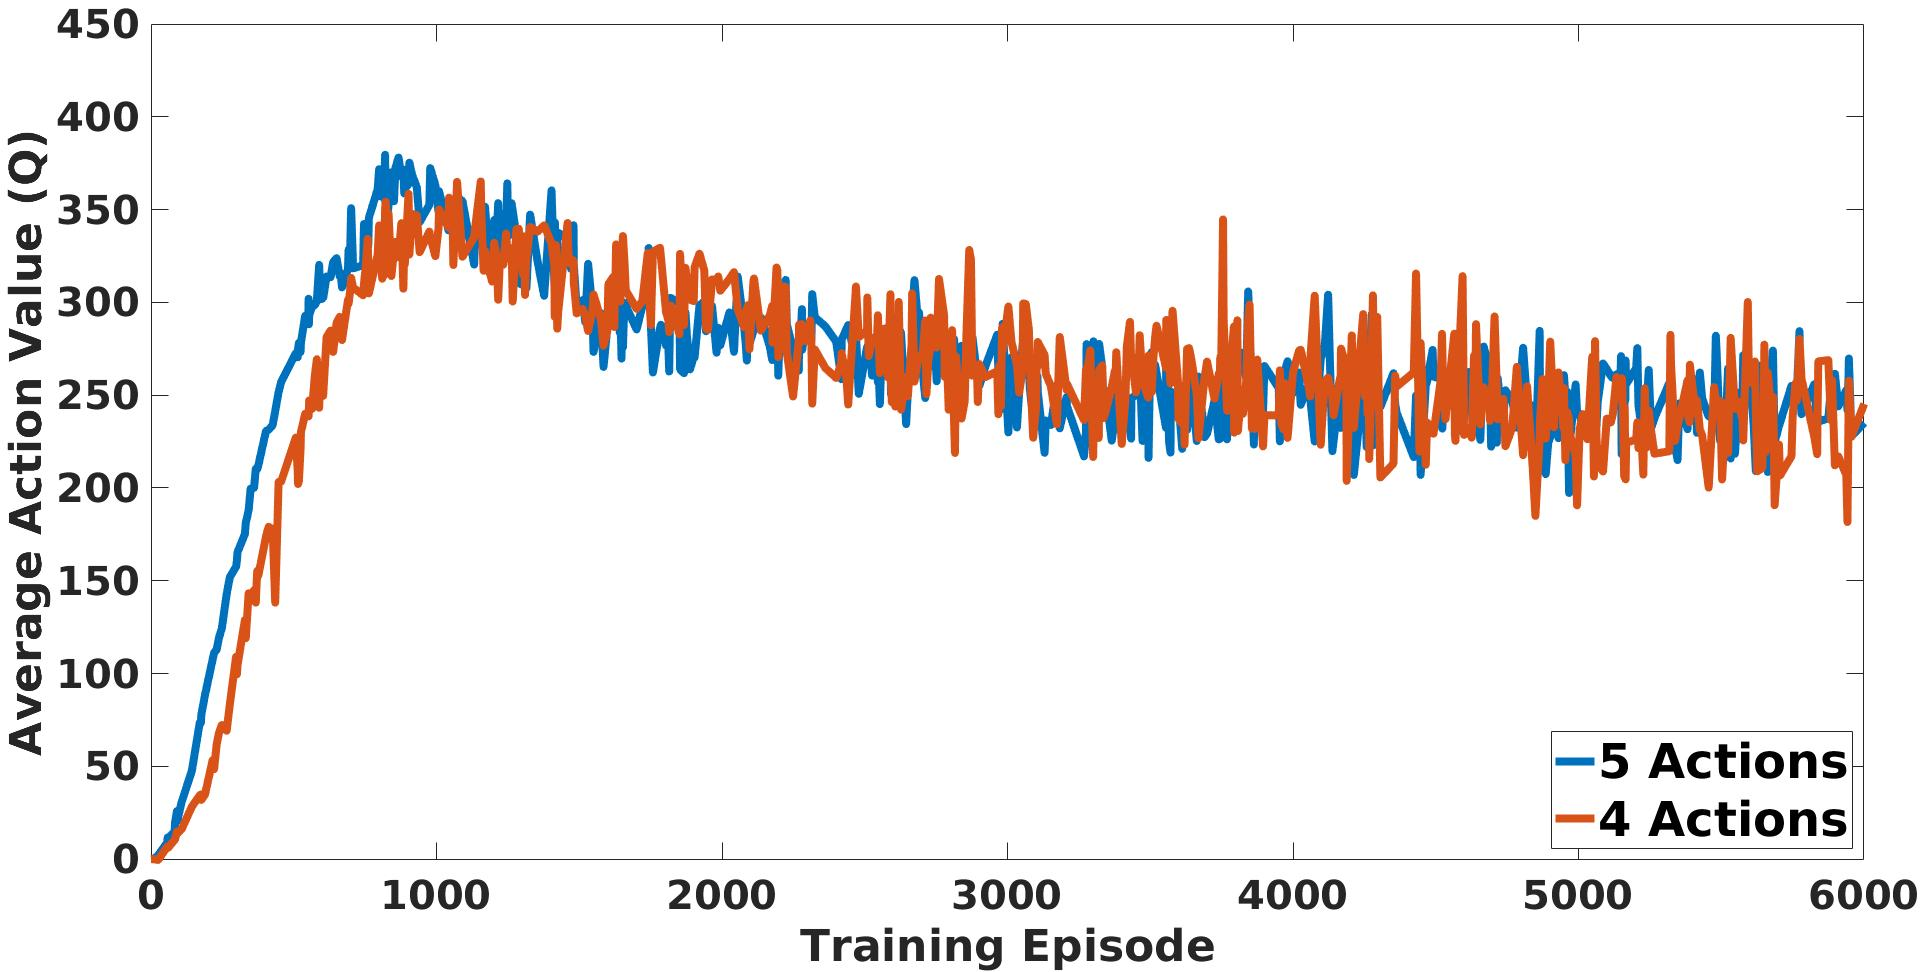
\includegraphics[width=0.6\textwidth]{Graphics/AveQ_action.jpg}
\caption[Average Action Values Action Space Comparison]{Average action
  values using four (orange) and five (blue) actions. 
Specific parameters are included in Table \ref{table: ActionSpace}}
\label{fig:action_test}
\end{figure}

\begin{figure}[h]
\centering
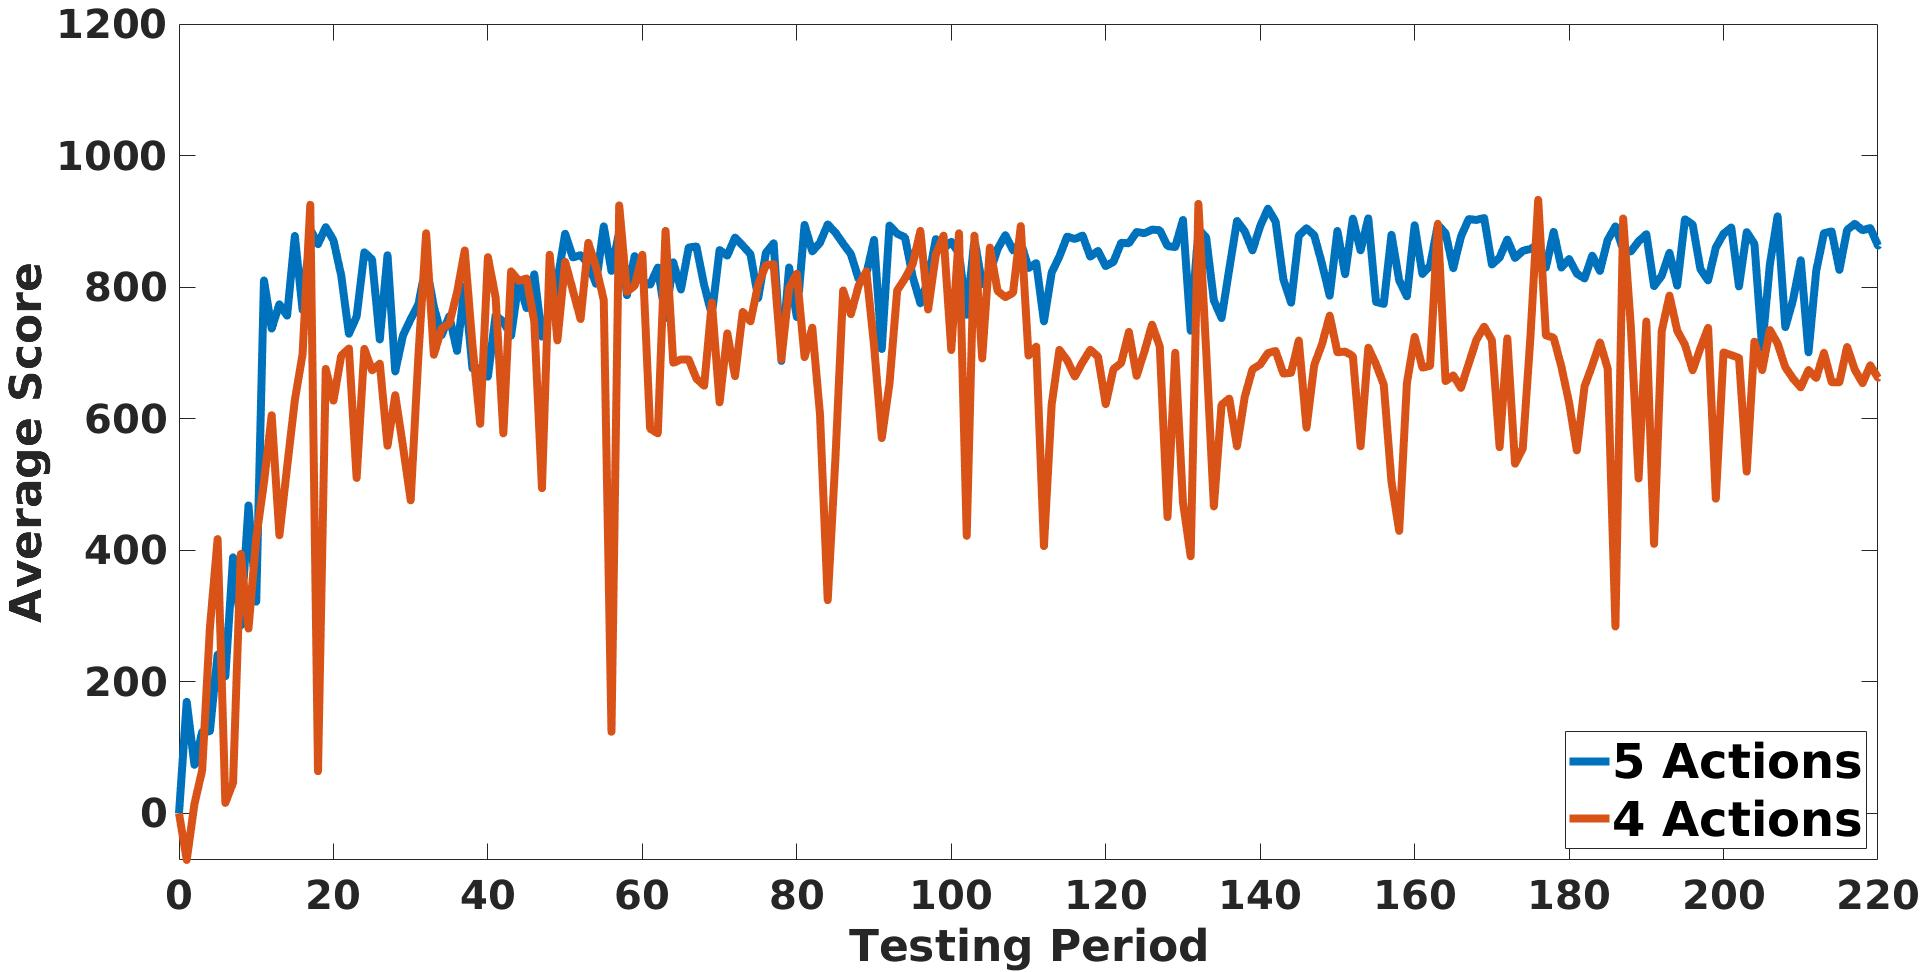
\includegraphics[width=0.6\textwidth]{Graphics/TestScore_action.jpg}
\caption[Average Test Score Action Space Comparison]{Average scores
  over five tests using four (orange) and five (blue) actions. 
Specific parameters are included in Table \ref{table: ActionSpace}}
\label{fig:action_aveq}
\end{figure}

As shown in Figure \ref{fig:action_aveq}, the model with five actions
achieves better average scores over five tests after 120 testing
periods. Hence we resolved to use five actions for models. 

\newpage
\section{Reward}
The nature of the reward signal from the environment greatly
influences the convergence and performance of RL models. Therefore, we
progressed to investigate the effect that rewards have on the
performance in the car racing game. As mentioned in section
\ref{sec1}, in the original game there are two different kinds of
rewards the agent can receive. For every tile the car visits, the
reward is 1000/N, where N is the total number of tiles on the track,
while for every frame passed, the reward is -0.1.  
\par
Intuitively, if the reward for visiting tiles is magnified, the agent
will tend to visit all tiles at the cost of possibly slowing down. If
the negative reward for one frame passed is magnified, the agent will
be encouraged to go faster while possibly missing some of the
tiles. Therefore, we experimented with changing the ratio and
magnitudes of positive and negative rewards.  
\par 
We trained models with six different pairs of positive and negative
rewards. We then tested the trained models on 100 random tracks and
compared the average scores and standard deviations. As shown in
Figure \ref{fig:rewardclip}, when the positive reward for visiting one
tile is fixed to 1, the performance worsens as the magnitude of the
negative reward decreases. When the negative reward is fixed to -0.1,
the performance varies when the positive reward changes from 20 to
1. We suspect there is a better reward pair, with positive reward
between 1 and 10 and negative reward being 0.1.  
\newpage
\begin{figure}[h!]
\centering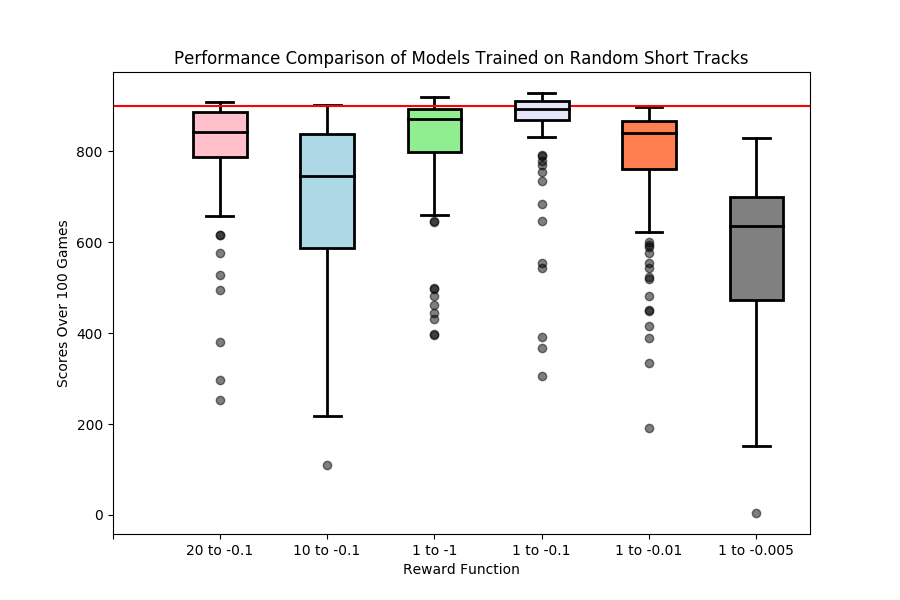
\includegraphics[scale=0.5,clip]{Graphics/performance_clip_reward.png}
\caption[Clip Reward Performance]{Performance of models with different
  reward ratios trained in the random short track
  environment.}\label{fig:rewardclip} 
\end{figure}

\endinput




% Chapter 6
\ifthenelse{\boolean{@twoside}}{\myclearpage}{}
\chapter{Performance Analysis}\label{Ch:Analyze}

After tuning the neural network structure and action space, we began to analyze the performance of our models. In section \ref{perf}, we explain the metrics we used for evaluating the model. We establish the baseline results in section \ref{base}. We compare the models with dropout to the baseline in the rest of this chapter. Note that in section \ref{solve}, we present a model that solved the CarRacing game challenge.

\section{Performance Metrics} \label{perf}
We used two metrics to evaluate the performance of our models. First, we allowed the model to play 100 games and computed the average score. Although the racetracks in these games were random, we used the same 100 racetracks for all tests in order to compare performance between models. We also compute the standard deviation of these 100 scores. This performance metric is based on the OpenAI challenge to achieve an average score of 900 or more over 100 games. 

\begin{figure}[H]
\centering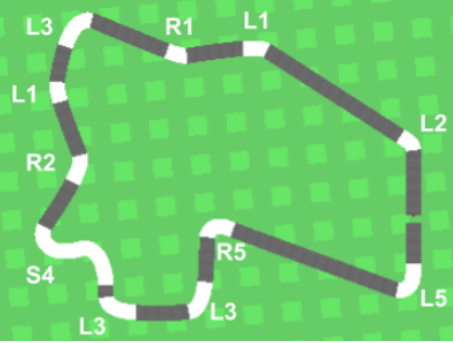
\includegraphics[scale=0.6,clip]
{Graphics/curve_characterization.png}
\caption[Curve Characterization]{An example of curve characterization}
\label{fig:curves}
\end{figure}

Second, we analyzed how the models performed on different curves in a racetrack. We developed a simple curve classification algorithm, which is demonstrated in Figure \ref{fig:curves}. Each curve is characterized as either as either a Left, Right, or S-shaped curve. An S-shaped curve is either a left turn followed by a right turn or a right turn followed by a left turn. Then, the steepness of the curve is ranked on a scale from 1 to 5, where 1 represents a very shallow curve and 5 represents a very steep curve. For example, L1 is a slight left curve and S4 is a fairly steep S-shaped curve. We compute the proportion of tiles that the agent visits for each class of curves. This performance metric is useful for understanding the strengths or weaknesses of a model as well as its ability to generalize to different curves.

\section{Baseline Results} \label{base}
We trained the algorithm on three environments and performed a baseline experiment. In the first environment, there was 1 predetermined racetrack that the agent interacts with during training.  In the second environment, there were 3 predetermined racetracks. In the third environment, the racetracks were generated randomly. The average score and standard deviation of testing these models over 100 random racetracks is shown in Table \ref{table:baseline_results}. 

\begin{table}[h]
\centering
\begin{tabular}{ m{4cm} | m{3cm}| m{3.5cm} } 
Model Environment & Average Score & Standard Deviation  \\
\hline 
1 Track & 849.99 & 78.72  \\
3 Track & 853.88 & 127.71  \\
Random Tracks & 854.83 & 107.14  \\
\end{tabular}
\caption{Baseline Performance over 100 random games}
\label{table:baseline_results}
\end{table}

The standard deviation of these test scores is fairly high because our current models are unable to perform well consistently. While testing these models, we observed that the algorithm struggled to generalize to different racetracks. For example, the model trained on a single fixed track catastrophically failed when it encountered a steep right curve during testing. We believe that this failure due to the fact that the model does not see any examples of steep right curves during training. This is an indicator that our algorithm is overfitting.

\section{Regularization with Dropout}
In order to prevent overfitting, we added dropout as a regularization technique to our neural network architecture by dropping out units at a rate of 30\% after the second convolutional layer of the neural network. We applied dropout to each of the three models tested in the baseline experiments in order to compare performance. The results of these experiments are shown in Table \ref{table:dropout}. 

\begin{table}[h]
\centering
\begin{tabular}{ m{4cm} | m{3cm}| m{3.5cm} } 
Model Environment & Average Score & Standard Deviation  \\
\hline 
1 Track & 894.38 & 24.5  \\
3 Tracks & 875.58 & 43.58 \\
Random Tracks & 887.39 & 24.65 \\
\end{tabular}
\caption{Performance for Dropout Rate 30\% over 100 random games}
\label{table:dropout}
\end{table}

When adding dropout to our neural network architecture, the average score over 100 games increased and standard deviation decreased in all three environments. The model achieved higher scores in the game more consistently. Hence, applying a dropout rate of 30\% improved the performance of our algorithm and came remarkably close to solving the OpenAI challenge of an average score of 900 over 100 random games.


\section{Curve Characterization}
We used the curve characterization method in order to determine whether applying dropout improved the ability of our algorithm to generalize to curves that were not seen during training. In particular, we analyzed the models that were trained on a single fixed track, because these models only saw a few curves durining training. Even though both models saw the same fixed track during training, the dropout model performed better on each class of steep curves. These results are demonstrated in Figure \ref{fig:dropout_curve}. These results indicate that using dropout allows the model to generalize better to curves it did not see during training. Thus, dropout has the potential to be an effective regularizer in deep reinforcement learning problems.

\begin{figure}[h!]
\centering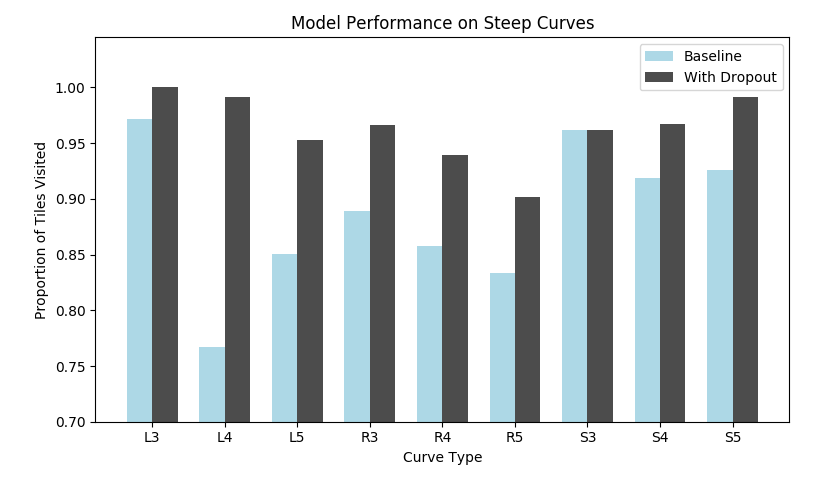
\includegraphics[scale=0.6,clip]
{Graphics/dropout_curve.png}
\caption[Curve Performance with Dropout]{Curve Performance with and without Dropout}
\label{fig:dropout_curve}
\end{figure}

\section{Solving Car Racing Game}\label{solve}
We then trained the neural network with dropping out units at a rate of 50\% to explore if higher dropout rate would improve the performance. The results of the experiments are shown in Table \ref{table:dropout_1}. 

\newpage
\begin{table}[h]
\centering
\begin{tabular}{ m{4cm} | m{3cm}| m{3.5cm} } 
Model Environment & Average Score & Standard Deviation \\ 
\hline 
3 Tracks & 906.67 & 23.6 \\
Random Tracks & 892.62 & 41.48 \\
\end{tabular}
\caption{Performance for Dropout Rate of 50\% over 100 random games}
\label{table:dropout_1}
\end{table}

Increasing the dropout rate from 30\% to 50\% increases the average score in all three environments. Using this method, we are able to achieve a score over 900 in the 3 Track environment, which successfully solves the OpenAI challenge.


\endinput



% Chapter 7
\ifthenelse{\boolean{@twoside}}{\myclearpage}{}
\chapter{Image Compression}\label{Ch:ImageProcessing}

GPUs have become increasingly common in machine learning due
to their rapid matrix multiplication. While we had access to
GPUs, the on-board memory was not sufficient to store the
images in the experience replay memory. Consequently, 
host-to-device transfer must occur to properly store all
images. In an effort to reduce the required memory, we
converted the eight-bit grayscale representation of 
images to binary images, reducing the memory consumption by
a factor of eight. The benefits of this compression
are twofold: foremost, we reduce the memory required,  and the 
agent learns to follow the road more closely. The latter is
discussed further in the next few sections.

\section{Edge Detection}
Upon completing a racetrack, we found that the car would not continue to drive on the road. This
suggested the agent learned to follow the tiles on the road; in their absence, the agent did 
not know to continue on the road to collect the missed tiles. While pursuing
tiles is a reasonable strategy for maximizing rewards in the game, this behavior is
at least detrimental in seeking missed tiles and at worst adverse in the context of real-life driving. 
To mend this, we altered the representation of the images fed into the network 
so that tiles were not visible to the agent.
An example of the altered image is given in Figure \ref{fig:canny_example}.

\begin{figure}[h]
\centering
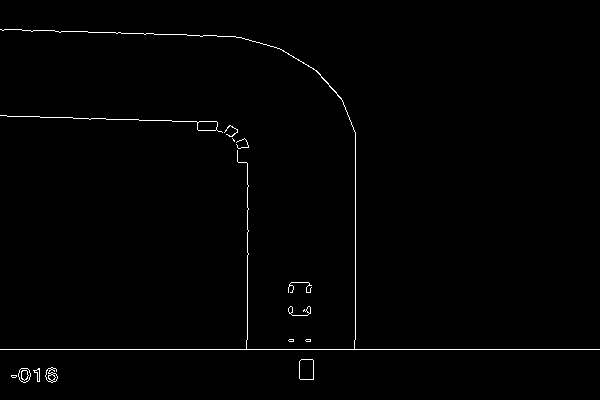
\includegraphics[width=0.6\textwidth]{Graphics/standard_gray_1_canny.png}
\caption{Edge detection compression}
\label{fig:canny_example}
\end{figure}

With this compression method, the
agent no longer sees tiles and must learn to stay on the road to receive rewards.
The method in question is a form of edge detection known as the Canny edge 
detection algorithm \cite{canny}. The next few sections provide an overview
of the Canny algorithm followed by a discussion of the 
performance of our
algorithm with this updated representation.

\newpage
\subsection{Canny Edge Detection}
The Canny algorithm consists of five main steps:

\begin{enumerate}[1.]
\item{Conversion from RGB to grayscale.}
\item{Noise suppression.}
\item{Gradient approximation.}
\item{Non-maximum edge suppression}
\item{Hysteresis thresholding}
\end{enumerate}

Each step is discussed in detail in the next few sections.

\subsection{RGB to Grayscale}
Several methods exist for converting a
red-green-blue (RGB) color image to grayscale, though
all reduce to taking a weighted average of each color channel. We used the 
conversion in Equation (\ref{eq:rgb2gray}), where $R,G,B$ represent the
red, green, and blue color channels (respectively) of the RGB image. 

\begin{align}\label{eq:rgb2gray}
Gray = .299R + .587G + .114B
\end{align}

An example of a grayscale conversion using Equation (\ref{eq:rgb2gray}) is given in 
Figure \ref{fig:rgb_to_grayscale}.

\begin{figure}[h]
\centering
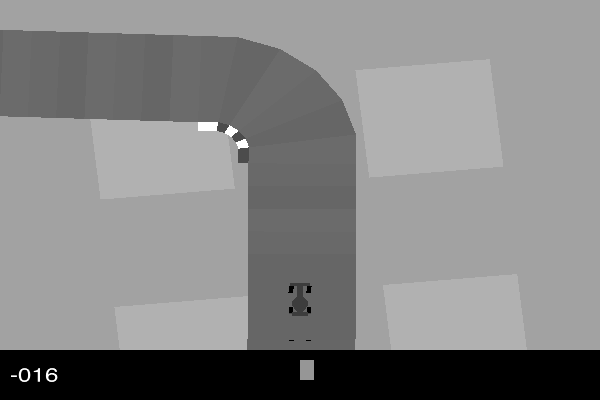
\includegraphics[width=0.6\textwidth]{Graphics/standard_gray_1.png}
\caption{Grayscale image representation}
\label{fig:rgb_to_grayscale}
\end{figure}

\subsection{Noise Suppression}
Edge detection is typically applied to images captured by digital cameras
and inherently exhibit some noise. For our purposes, `noise' refers to
regions in the image that are not crucial in the agent's learning how
to navigate the tracks. Such regions are the tiles and grass squares
visible in Figure \ref{fig:rgb_to_grayscale}.

A common technique used to 
suppress noise is image smoothing where pixel values are replaced
by a weighted average of its neighbors. This weighted average computation
is typically performed via convolution. Given two continuous functions 
$f,g$ with bounded support $[0, \infty)$, the convolution of $f$ and $g$
gives a third function and is defined as

\begin{align}\label{eq:cont_conv}
(f*g)(t) &= \int_0^t f(\tau)g(t-\tau)d\tau.
\end{align}

For discrete functions, the convolution is given by

\begin{align}\label{eq:disc_conv}
(f*g)(t) &= \sum_{\tau=0}^t f(\tau)g(t-\tau).
\end{align}

\par
To be more precise, let $f$ above denote the grayscale image obtained
using Equation (\ref{eq:rgb2gray}). $g$ will then be a two-dimensional matrix,
called a kernel, that determines how much weight to give to neighboring
pixels. We used the $3\times 3$ Gaussian kernel given below

\begin{align*}
g &=
\begin{bmatrix}
0.0751 & 0.1238 & 0.0751 \\
0.1238 & 0.2042 & 0.1238 \\
0.0751 & 0.1238 & 0.0751
\end{bmatrix}
\end{align*}

which can be found by taking the matrix below and dividing so that the
matrix entries sum to 1; $h$ here refers to the 
bivariate Gaussian density 
$\mathcal{N}\left([0,0],\begin{bmatrix} 1 & 0  0 & 1 \end{bmatrix}\right)$.

\begin{align*}
\begin{bmatrix}
h(-1,-1) & h(0,-1) & h(1,-1) \\
h(-1,0) & h(0,0) & h(1,0) \\
h(-1, 1) & h(0, 1) & h(1,1)
\end{bmatrix}.
\end{align*}

Let $h$ now be the output of convolving the image $f$ with kernel $g$, then
$h(m,n$) is given by

\begin{align}\label{eq:img_conv}
h(m,n) &= \sum_{k=-1}^{1} \sum_{l=-1}^{1} f(m-k,n-l)g(k,l)
\end{align}

where $g$ is indexed such that the top left entry is entry $(-1,-1)$
and its bottom right entry is $(1,1)$. $h$ now represents the smoothed image;
this operation is typically referred to as a Gaussian blur. 

\subsection{Gradient approximation}
For our purposes, an edge refers to a change in pixel intensity. Change in 
functions is typically quantified by differentiation; the same applies to
images.
Having smoothed the image using Equation \ref{eq:img_conv}, edges are identified
by computing this image's gradient. Letting $f$ be a differentiable function,
its derivative at $x$, $f'(x)$, is defined as

\begin{align}\label{eq:derivative_def}
f'(x) &= \lim_{h \to 0} \frac{f(x+h) - f(x)}{h}.
\end{align}

For a small enough $h$, $f'(x)$ can be approximated using the forward 
difference approximation in Equation (\ref{eq:finite_diff_forward}).

\begin{align}\label{eq:finite_diff_forward}
f'(x) \approx \frac{f(x+h) - f(x)}{h}
\end{align}

For images, a more accurate derivative approximation is the central difference
defined in Equation (\ref{eq:finite_diff_central}).

\begin{align}\label{eq:finite_diff_central}
f'(x) \approx \frac{f(x+.5h) - f(x-.5h)}{h}
\end{align}

An image is two-dimensional and hence has derivatives along two axes, which
we call $x$ and $y$.
Thus, given a signal such as that in Table \ref{table:1dSignal}--which can be
interpreted as the row of an image--it can be differentiated using Equation
(\ref{eq:finite_diff_central}). 

\begin{table}
\centering
\begin{tabular}{|c|c|c|c|c|}
\hline 
40 & 40 & 200 & 240 & 100 \\
\hline
\end{tabular}
\caption{1-dimensional signal}
\label{table:1dSignal}
\end{table}

For example, to estimate the derivative
of the signal at the third pixel value of 200, we compute
$\frac{240-40}{2} = 100$. 

Padding the image with zeros allows us to perform the operation above to
every pixel in the signal. Up to scaling by a constant, this operation is computationally equivalent to convolving the signal with the
kernel $[-1, 0, 1]$. Thus to obtain the gradient along the $x$ direction
of an image, we simply need to convolve it with the kernel $[-1, 0 ,1]$. 
This operation outputs a grayscale image with edges most prominent along
the original image's $x$ direction; however, this also introduces `false 
edges'--edges that may not necessarily be edges of interest. To remedy
this, we blur the outputted image with a smoothing filter. In particular,
we will convolve the gradient approximation with the kernel 
$[1, 2, 1]^T$. We smooth along the y-axis so that false edges parallel
to the x-axis are averaged. Thus, to obtain the gradient along the
x-direction of the smoothed image, $h$, given by Equation (\ref{eq:img_conv}), we 
compute

\begin{align}\label{eq:grad_x_1}
I_x &= h * 
\begin{bmatrix}
-1 & 0 & 1
\end{bmatrix} *
\begin{bmatrix}
1  2  1
\end{bmatrix}.
\end{align}

The convolution operation is associative, allowing us to first convolve
the filters in Equation (\ref{eq:grad_x_1}) to obtain

\begin{align}\label{eq:grad_x_2}
I_x &= h * 
\begin{bmatrix}
-1 & 0 & 1 \\
-2 & 0 & 2 \\
-1 & 0 & 1
\end{bmatrix}
\end{align}

where the filter on the right of Equation (\ref{eq:grad_x_2}) is called the Sobel 
filter. In literature, the filter above may be presented as having the
negative values on the rightmost column and the positive values on the
leftmost column; we prefer our representation as it illustrates how the
kernel arises. Moreover, the sign of the kernel is not imperative as
we are interested in magnitudes. 

We can similarly obtain the gradient along the y-axis by convolving with
the transpose of the Sobel kernel given in Equation (\ref{eq:grad_x_2}):

\begin{align}\label{eq:grad_y_1}
I_y &= h * 
\begin{bmatrix}
-1 & -2 & -1 \\
0 & 0 & 0 \\
1 & 2 & 1
\end{bmatrix}.
\end{align}

Having obtained the gradients along the x and y axes, the magnitude of
the gradient, $I$, can be obtained by computing

\begin{align}\label{eq:gradient_mag}
I &= \sqrt{I_x^2 + I_y^2}.
\end{align}

Similarly, the direction of the gradient, $\theta$, can be obtained by
computing

\begin{align}\label{eq:gradient_direc}
\theta &= \textrm{arctan}\left(\frac{I_y}{I_x}\right).
\end{align}

At this juncture, $I$ in Equation (\ref{eq:gradient_mag}) represents the edges of
the image, though it contains false edges. The next two sections discuss
methods to suppress these edges using $\theta$ and hysteresis 
thresholding.

\subsection{Non-Maximum Edge Suppression}
By smoothing the original grayscale image, we have changed the values
of the pixels such that we will ultimately be able to remove them in
the final step of the Canny algorithm. At this stage, it is possible
that the unwanted edges are still present in $I$. Indeed, this is 
corroborated by visualizing $I$ in Figure \ref{fig:thick_edges_example}
where the tile and grass edges are clearly visible. These will be
removed in the next step of the Canny algorithm, but this image
reveals another potential issue: the edges are very thick. This
step of the edge detection algorithm aims to thin these edges via
a method known as non-maximum edge suppression.

\begin{figure}[h]
\centering
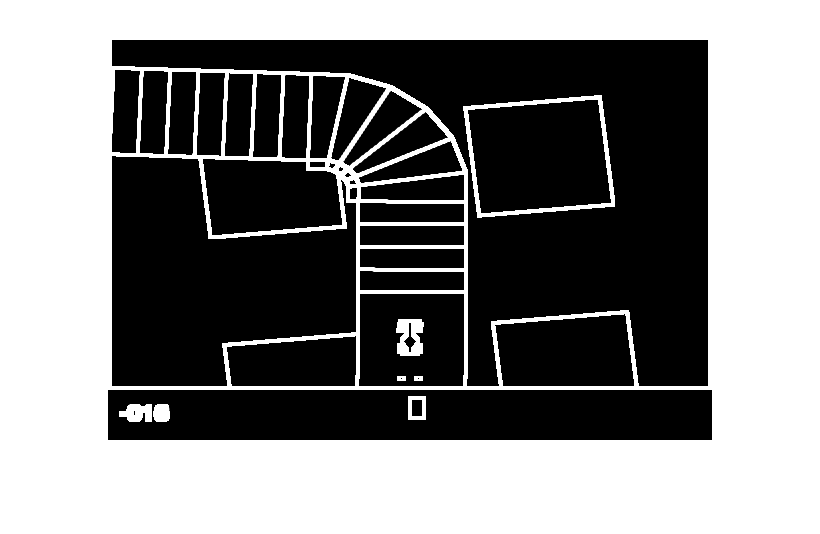
\includegraphics[width=0.6\textwidth]{Graphics/thick_edges_example.png}
\caption{Thick edges}
\label{fig:thick_edges_example}
\end{figure}

This technique goes through every pixel in $I$ and compares the pixel
value to the value of its neighbors; if the pixel value is larger
than those of its neighbors, it is kept, otherwise it is set to 0. 
If $(i,j)$ represents the pixel in question, its `neighbors' are defined
to be the pixels parallel to the direction of $(i,j)$ where the
direction is given by the gradient direction at $(i,j)$--that is, 
$\theta(i,j)$. 

\par
Images are discrete objects and each pixel is surrounded by eight
potentially neighboring pixels. Thus, the direction of a pixel's gradient
must be discretized into eight possible directions. As such, every entry
in $\theta$ will be binned into eight possible directions: north to south, 
south to north, east to west, west to east, southwest to northeast, 
northeast to southwest, northwest to southeast, and southeast to 
northwest. A diagram illustrating these directions is given in 
Figure \ref{fig:disc_grad_dir}. 

\begin{figure}
\centering
\begin{subfigure}{.5\textwidth}
  \centering
  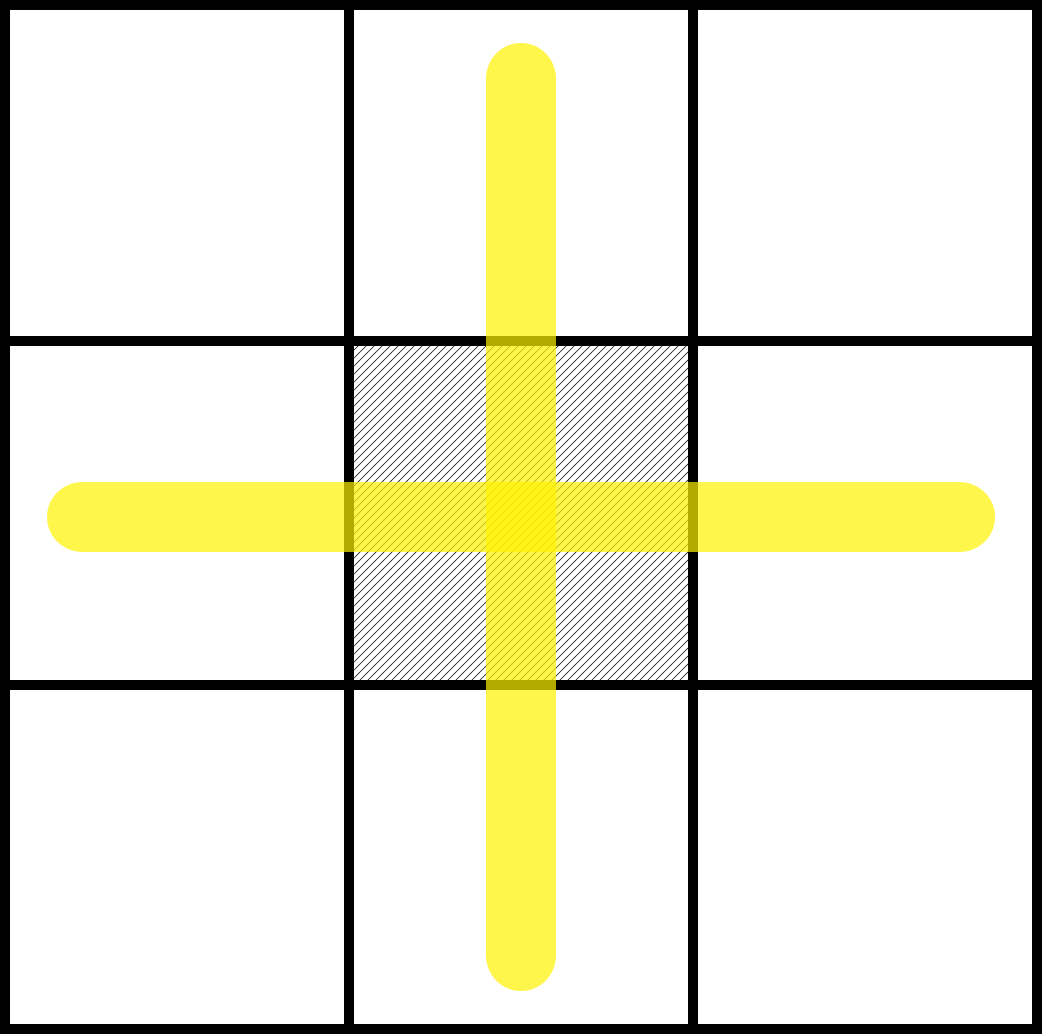
\includegraphics[width=.4\linewidth]{Graphics/disc_grad_dir_cross.png}
  \caption{N to S, W to E}
  \label{fig:disc_grad_dir_cross}
\end{subfigure}%
\begin{subfigure}{.5\textwidth}
  \centering
  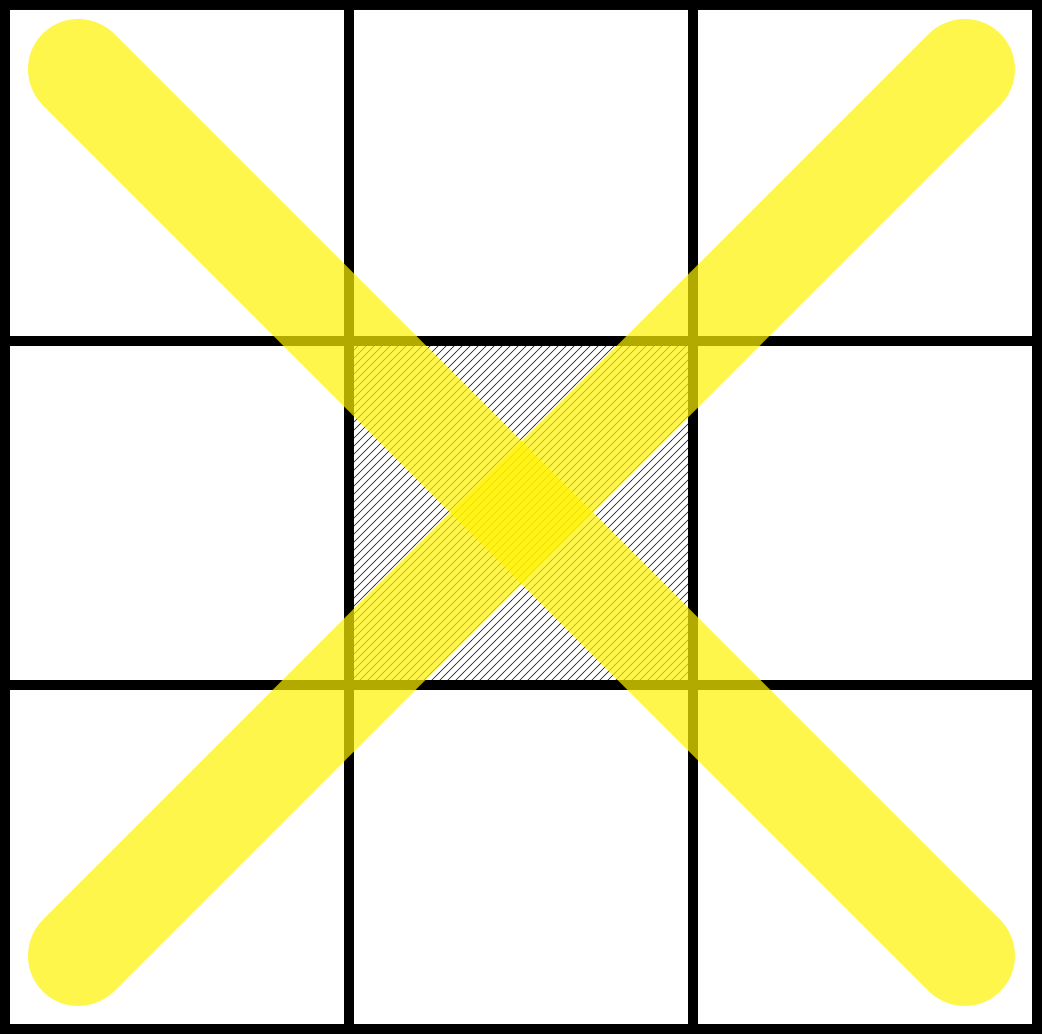
\includegraphics[width=.4\linewidth]{Graphics/disc_grad_dir_diag.png}
  \caption{NW to SE, SW to NE}
  \label{fig:disc_grad_dir_diag}
\end{subfigure}
\caption{Discretized gradient directions}
\label{fig:disc_grad_dir}
\end{figure}

This diagram depicts a clear redundancy: directions can be discretized
into four bins. As such, gradient directions will be classified as one of:
north to south, west to east, northwest to southeast, and southwest to 
northeast. The discretization is performed as shown in Table 
\ref{table:grad_discretization}, where the left column is the value
of $\theta$ in degrees and the right column is the corresponding bin;
the notation $(a,b)$ denotes the set of numbers in the range from $a$
to $b$. 

\begin{table}
\centering
\begin{tabular}{c|c}
Angle & Bin \\
\hline
(0, 22.5) $\cup$ (157.5, 202.5) $\cup$ (337.5, 360) & W to E \\
(22.5, 67.5) $\cup$ (202.5, 247.5) & SW to NE \\
(67.5, 112.5) $\cup$ (247.5, 292.5) & N to S \\
(112.5, 157.5) $\cup$ (292.5, 337.5) & NW to SE
\end{tabular}
\caption{Gradient direction binning}
\label{table:grad_discretization}
\end{table}

Once the gradient directions have been discretized, every pixel in
$I$ is compared to its neighbors. The neighbors of a pixel are determined
by the direction of its gradient. The neighbors for every gradient
direction is given in Figures \ref{fig:disc_grad_dir_neighbors_1}
and \ref{fig:disc_grad_dir_neighbors_2}. 

\begin{figure}[h!]
\centering
\begin{subfigure}{.5\textwidth}
  \centering
  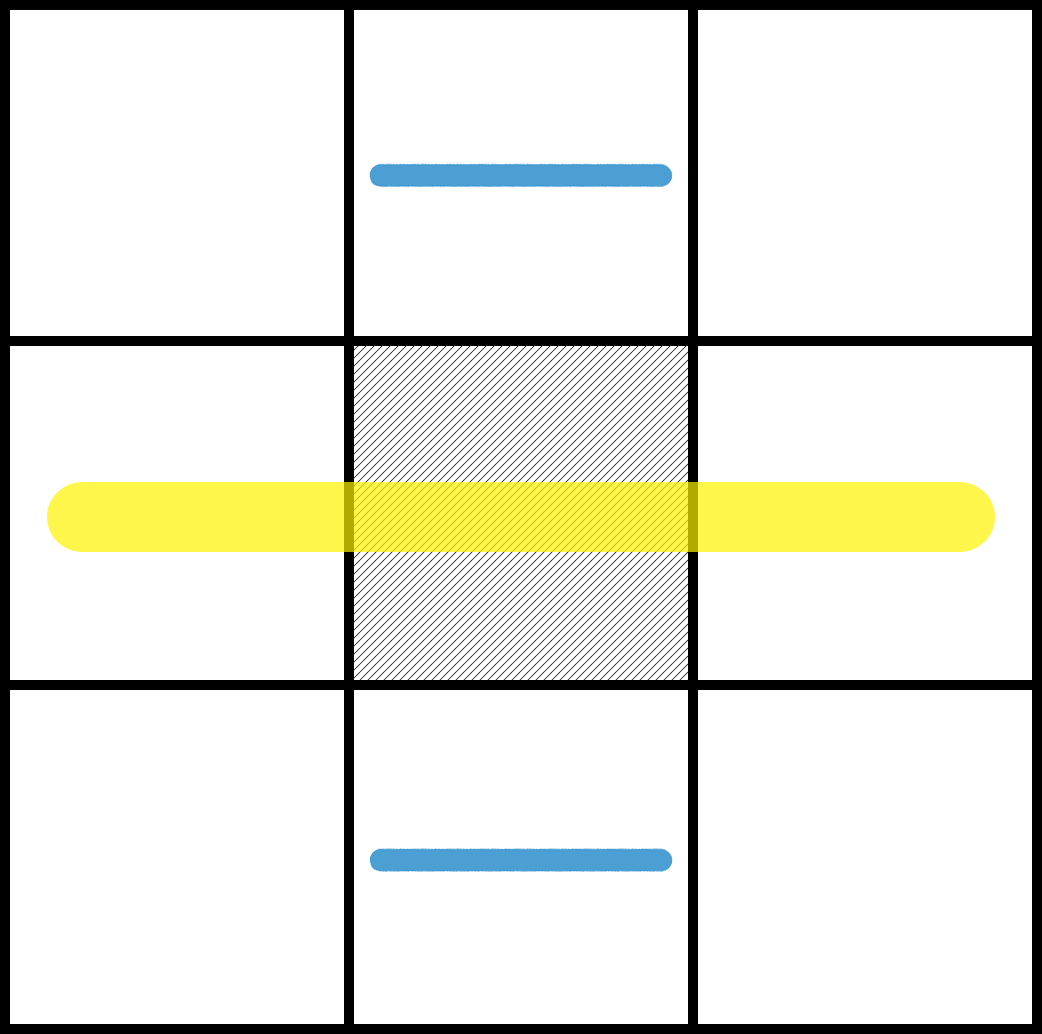
\includegraphics[width=.4\linewidth]{Graphics/disc_grad_dir_neighb_horizontal.png}
  \caption{W to E neighbors}
  \label{fig:disc_grad_dir_horiz}
\end{subfigure}%
\begin{subfigure}{.5\textwidth}
  \centering
  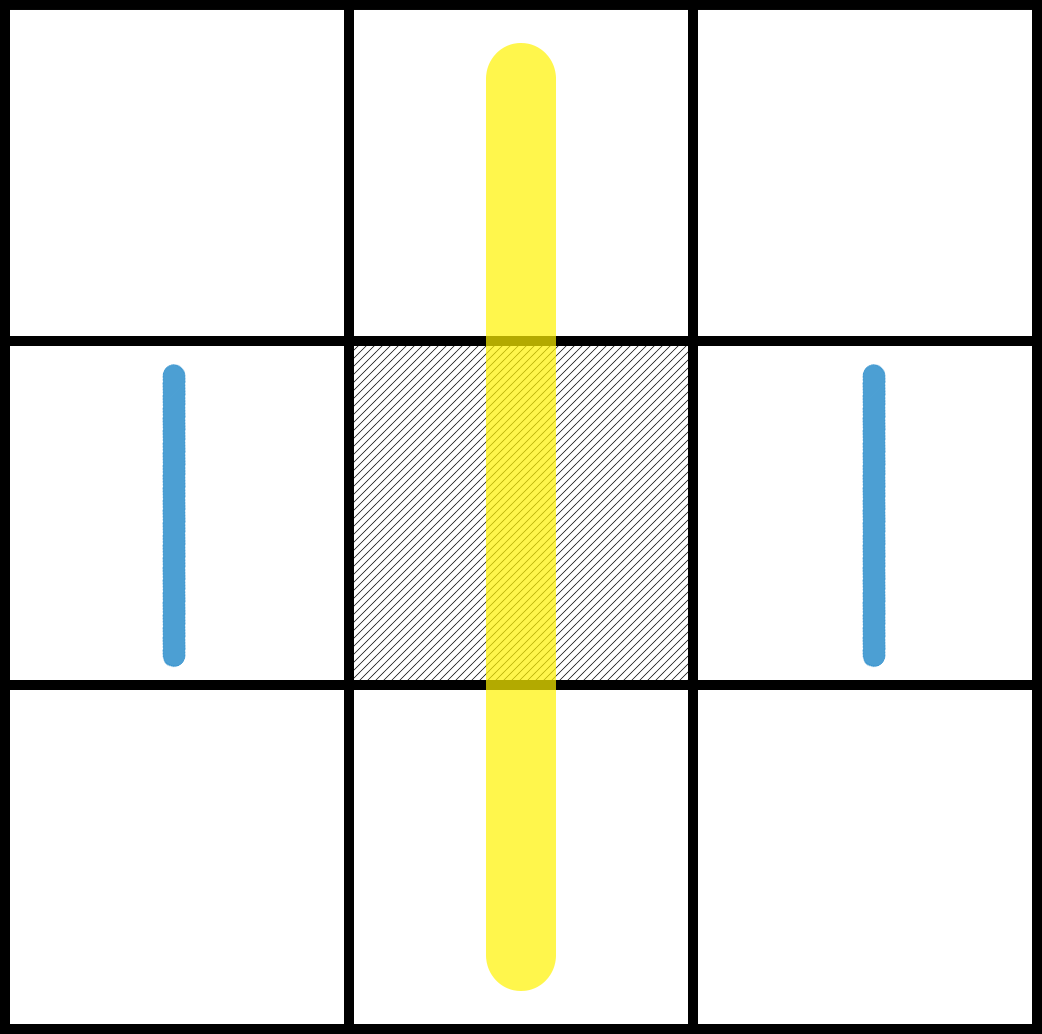
\includegraphics[width=.4\linewidth]{Graphics/disc_grad_dir_neighb_vertical.png}
  \caption{N to S neighbors}
  \label{fig:disc_grad_dir_vert}
\end{subfigure}
\caption{Discretized gradient directions}
\label{fig:disc_grad_dir_neighbors_1}
\end{figure}

\begin{figure}[h!]
\centering
\begin{subfigure}{.5\textwidth}
  \centering
  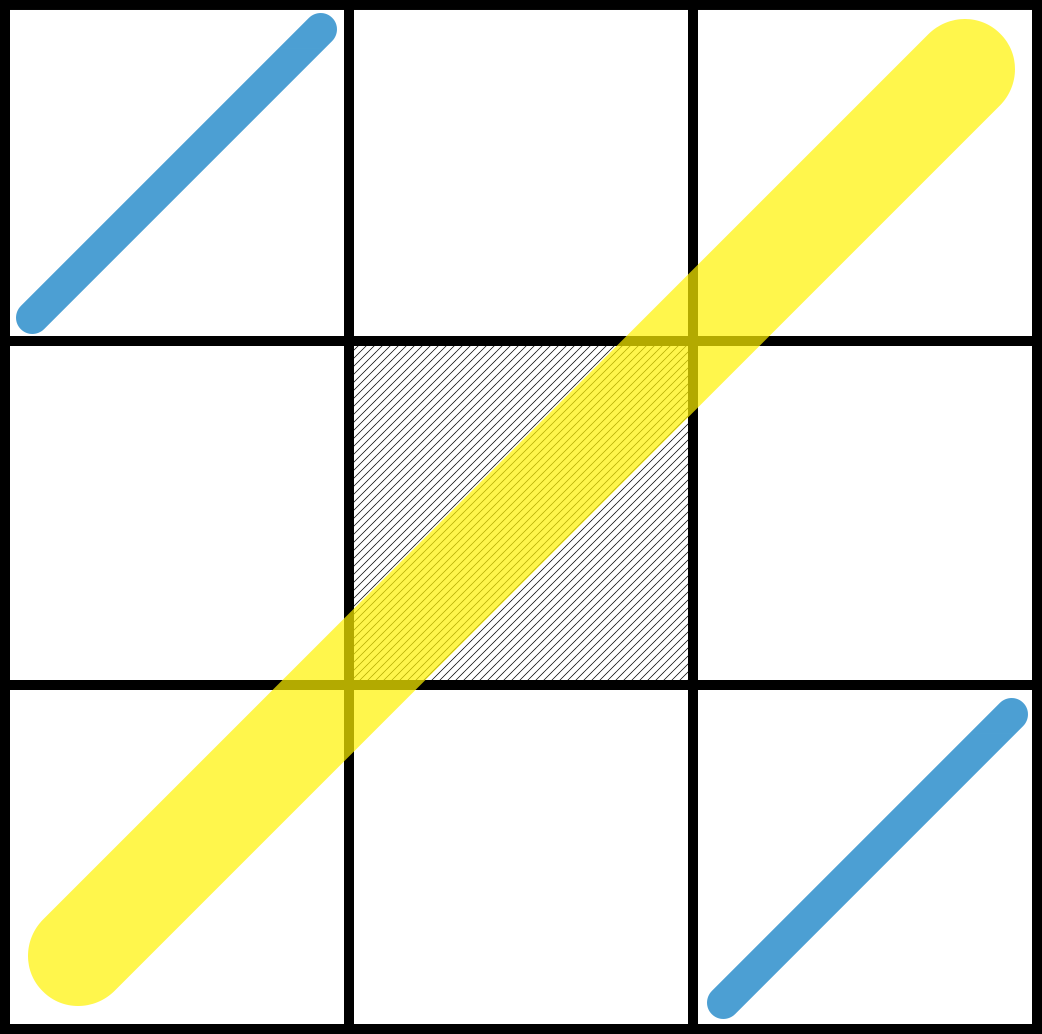
\includegraphics[width=.4\linewidth]{Graphics/disc_grad_dir_diag_1.png}
  \caption{SW to NE neighbors}
  \label{fig:disc_grad_dir_diag_1}
\end{subfigure}%
\begin{subfigure}{.5\textwidth}
  \centering
  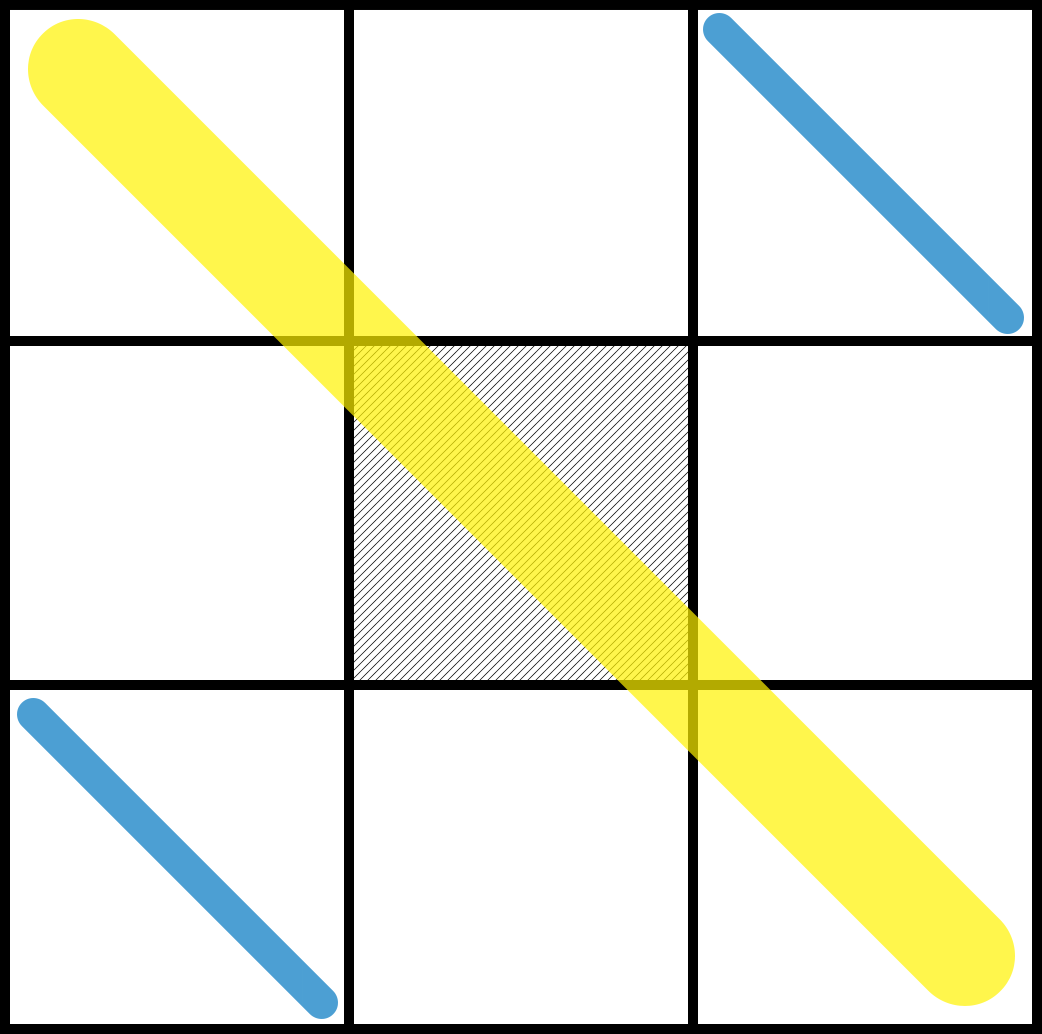
\includegraphics[width=.4\linewidth]{Graphics/disc_grad_dir_diag_2.png}
  \caption{NW to SE neighbors}
  \label{fig:disc_grad_dir_diag_2}
\end{subfigure}
\caption{Discretized gradient directions}
\label{fig:disc_grad_dir_neighbors_2}
\end{figure}

For example, if pixel $(i,j)$ has a gradient direction of SW to NE
as in Figure \ref{fig:disc_grad_dir_diag_1}, then the
neighbors of $(i,j)$ are pixels $(i-1,j-1)$ and $(i+1,j+1)$. We then
compare the value of pixel $(i,j)$ to its neighbors and set it to zero
if its value is less than those of its neighbors, otherwise its value
remains the same. 

After performing the operation outlined above, we obtain an image
similar to that in Figure \ref{fig:thick_edges_example}, though
now the edges have been thinned as shown in Figure 
\ref{fig:thin_edges_example}.

\begin{figure}[h!]
\centering
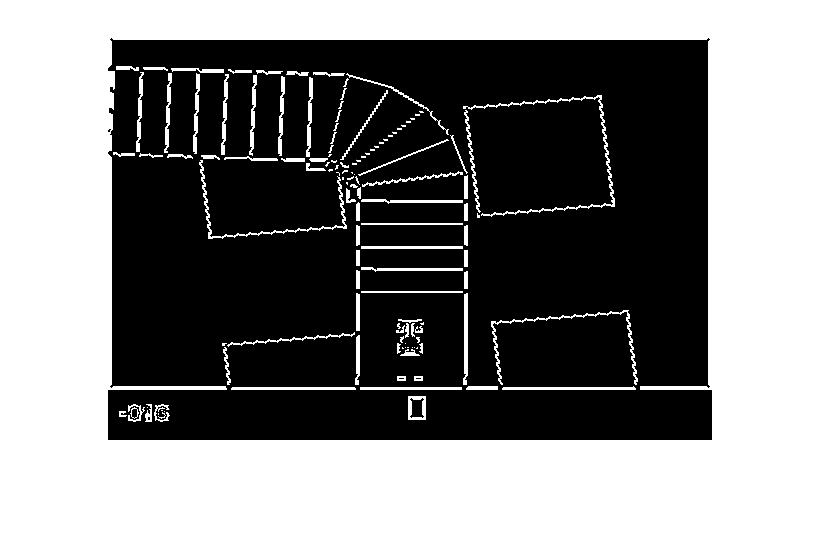
\includegraphics[width=0.6\textwidth]{Graphics/thinned_edges_example.png}
\caption{Thin edges}
\label{fig:thin_edges_example}
\end{figure}

\subsection{Hysteresis Thresholding}
After performing non-maximum edge suppression via the procedure outlined
above, the final step of the Canny edge detection algorithm is to remove
edges that are deemed insignificant. More precisely, we will introduce
two parameters $a,b \in \{0,1,2,\ldots, 255\}$ $a > b$ known as
thresholds. Then, every pixel in the thinned image will be compared to 
these thresholds: values less than $b$ will be discarded (set to zero), 
and values greater than $a$ will be kept (set to one). Values 
between $a$ and $b$ will be kept only if the pixel is connected to
an edge with a pixel value greater than $a$. More precisely, 
if the value of pixel $(i,j)$ is between $a$ and $b$, we will look
at its neighbors (as determined by the gradient direction) and 
set the value of pixel $(i,j)$ to one if one of its neighbors has
a value greater than $a$, otherwise it will be set to zero.

For our algorithm we used the thresholds $a = 150$ and $b=250$. 
Applying hysteresis thresholding to Figure \ref{fig:thin_edges_example}
yields the image in Figure \ref{fig:canny_example}.

\subsection{Edge Detection Performance}
In writing, feeding the output of the compressed edge detected image
offers several benefits: the agent learns to stay on the road and the
required memory decreases by a factor of eight. However, it is 
important to verify these claims. The orange curve in Figure 
\ref{fig:aveQ_edge} plots the average Q-function of our algorithm when 
the images fed are those passed through the edge detection algorithm; the
blue line depicts the average Q-function when the images are simply 
grayscale images. In particular, both models were trained on three
fixed tracks and tested on random ones. Both methods converge to similar 
values, suggesting the algorithm retains its generalizability. Moreover,
the orange curve in Figure \ref{fig:test_edge} depicts the average
training score for the edge detection algorithm as compared to the
grayscale algorithm (in blue); there is no evidence suggesting the
performance of the algorithm is compromised. 


In short, by first passing the images output by the environment through
an edge detection compression, we are able to reduce the amount of 
memory required for training, and retain the performance obtained 
without compressing the image. 

\begin{figure}[]
\centering
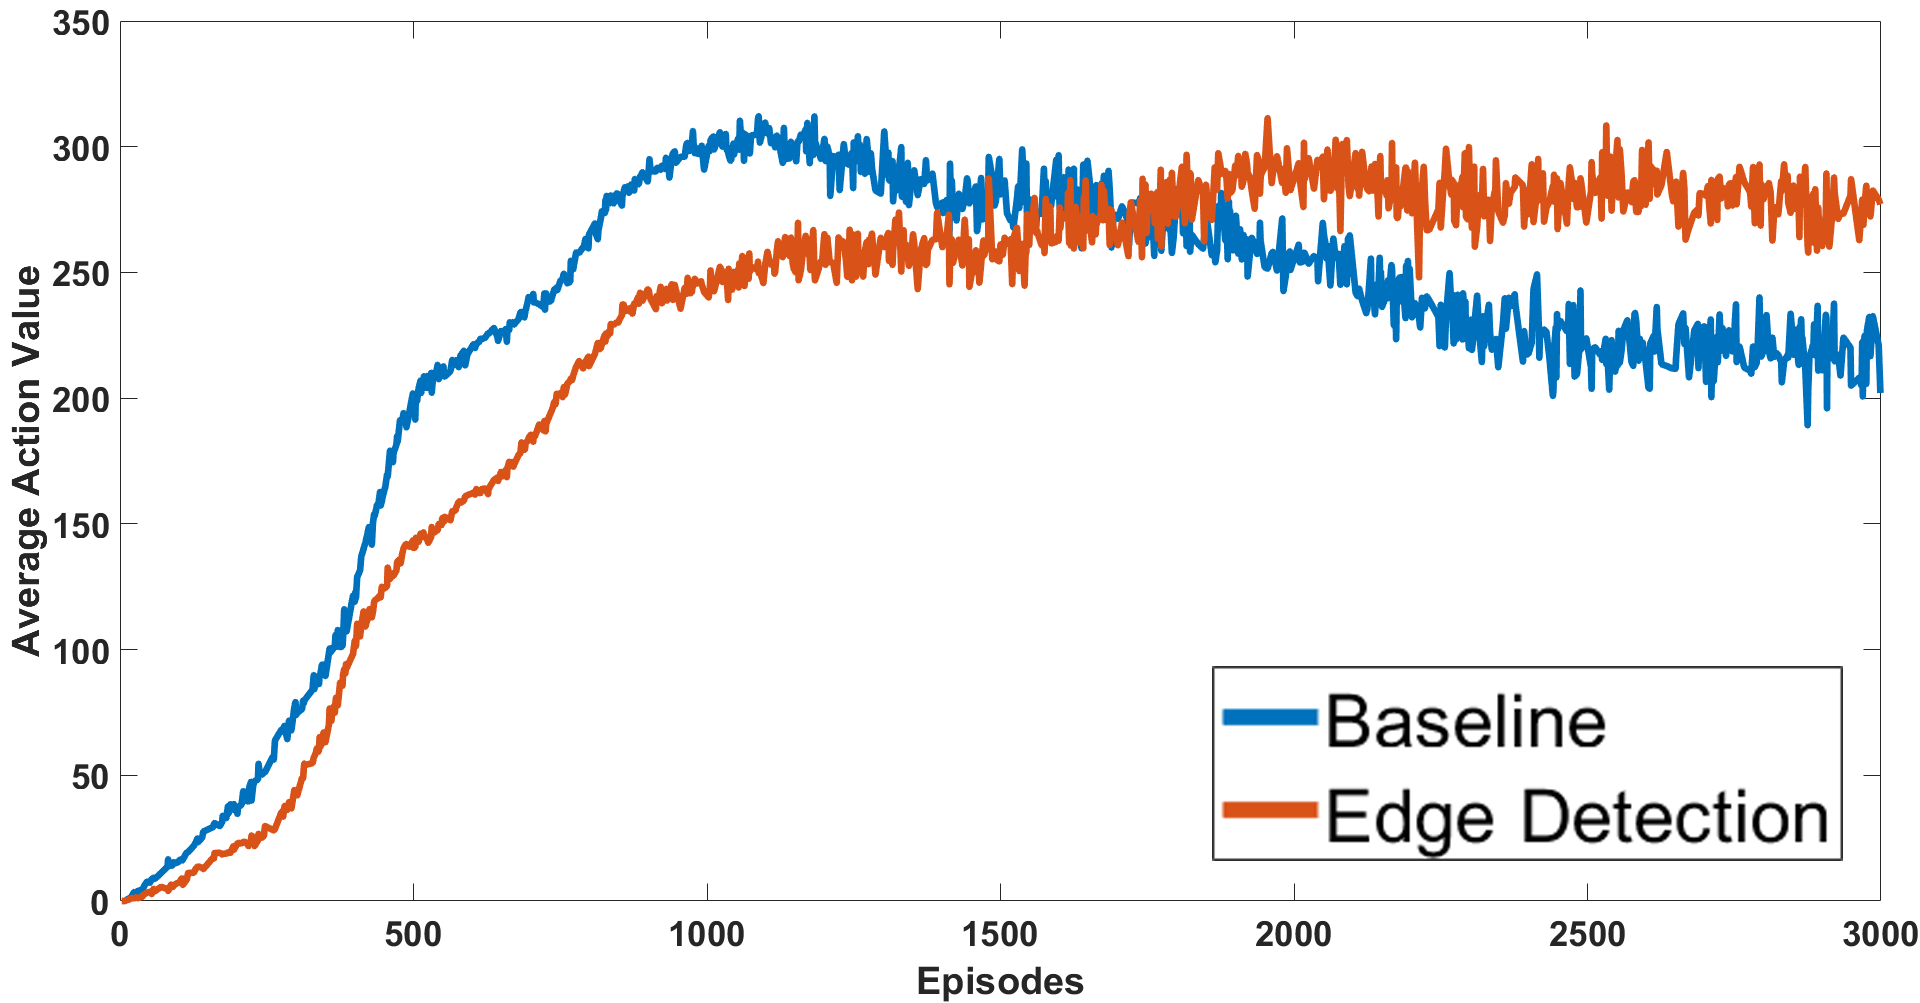
\includegraphics[width=.6\linewidth]{Graphics/edge_perf_q_large.png}
\caption{Average Q-value for edge detection}
\label{fig:aveQ_edge}
\end{figure}

\begin{figure}[]
\centering
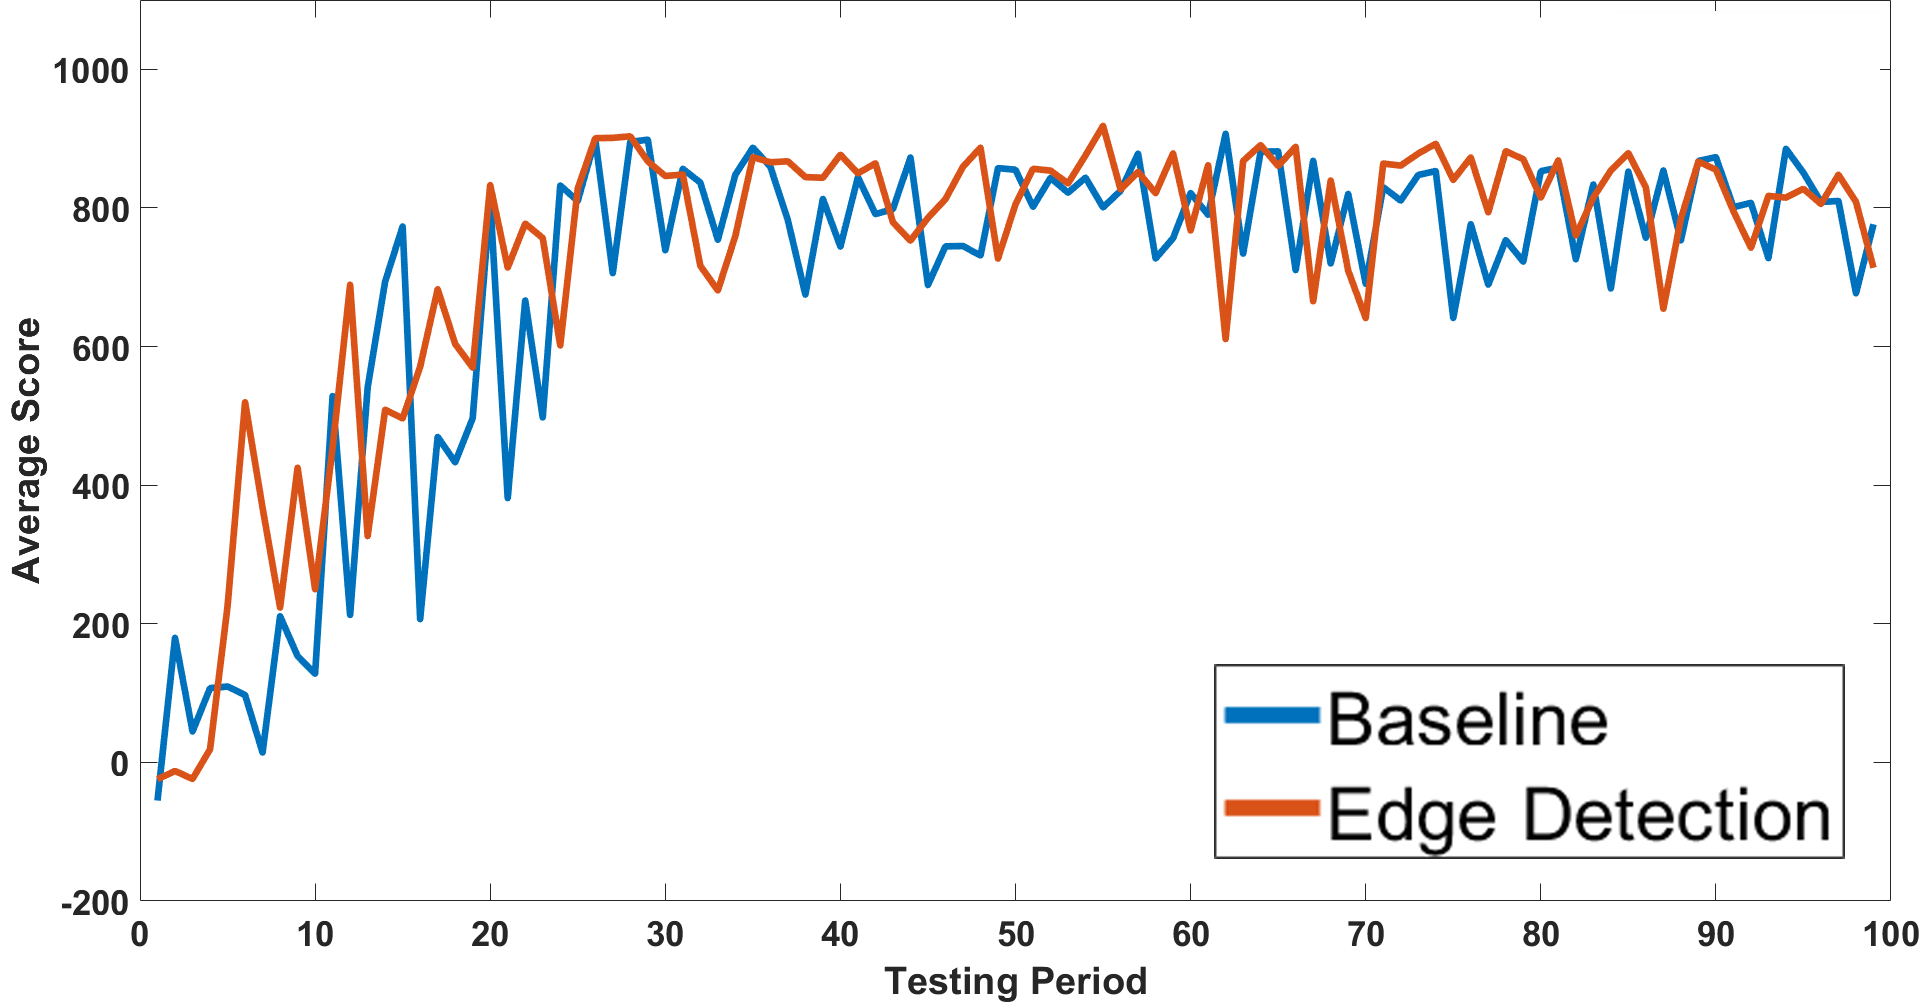
\includegraphics[width=.6\linewidth]{Graphics/edge_perf_score_large.png}
\caption{Average training score for edge detection}
\label{fig:test_edge}
\end{figure}

\newpage
\section{Grass Detection}
A common behavior exhibited by the agent is cutting corners as shown
in Figure \ref{fig:cut_corner}. 

\begin{figure}[h]
\centering
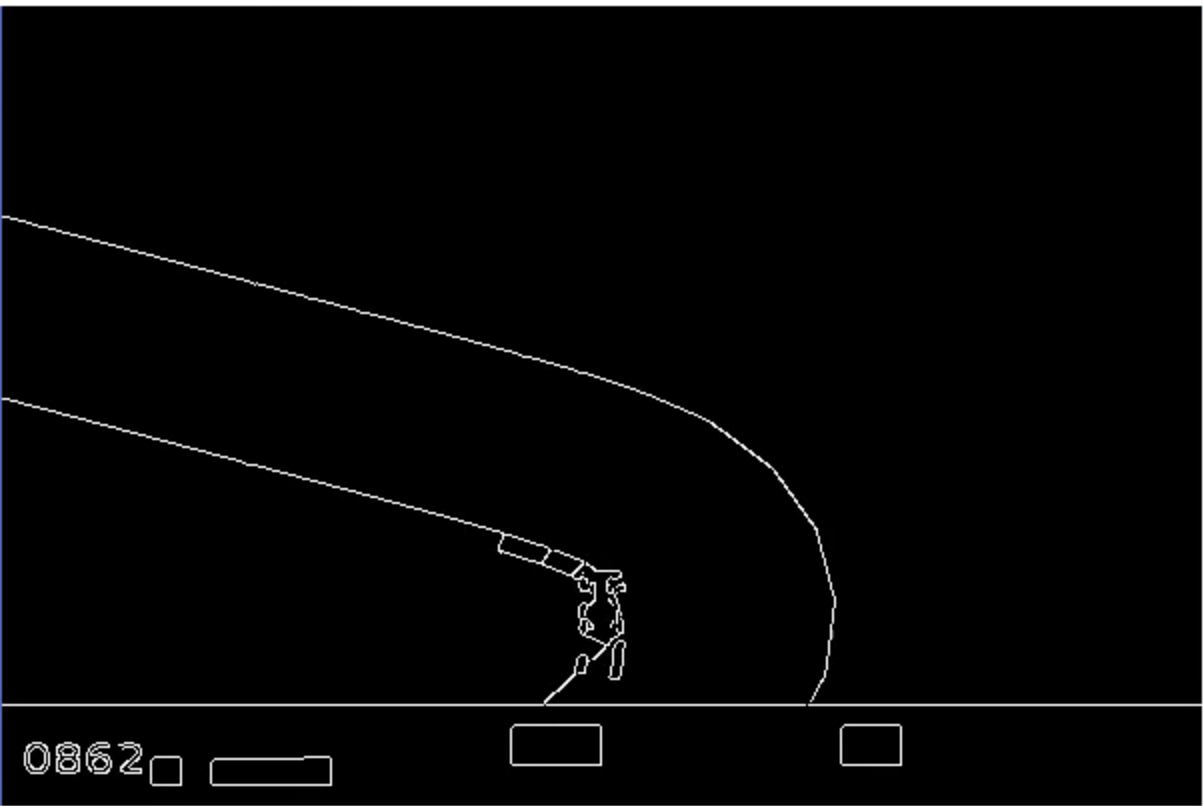
\includegraphics[width=0.6\textwidth]{Graphics/cut_corner.png}
\caption{Agent cuts corners}
\label{fig:cut_corner}
\end{figure}

Moreover, as commonly seen in professional race car driving, the 
car lingers along the right edge of the track to easily make left turns.
Consequently, when presented with a right turn, the agent has trouble
making it and often misses tiles. Both of these issues can be resolved
if the agent learns to stay out of the grass. While it is possible that
over time the agent will learn to stay out of the grass, the long training
time is undesirable. As such, we implemented a form of grass detection
so that the agent receives a negative reward while training to learn
to avoid the grass. The grass detection implementation is very simple: we 
simply crop a $13 \times 11$ rectangle around the car and count the
number of green pixels. If the number of green pixels is larger than 44, 
then we say the car is in the grass. 

\begin{figure}[]
\centering
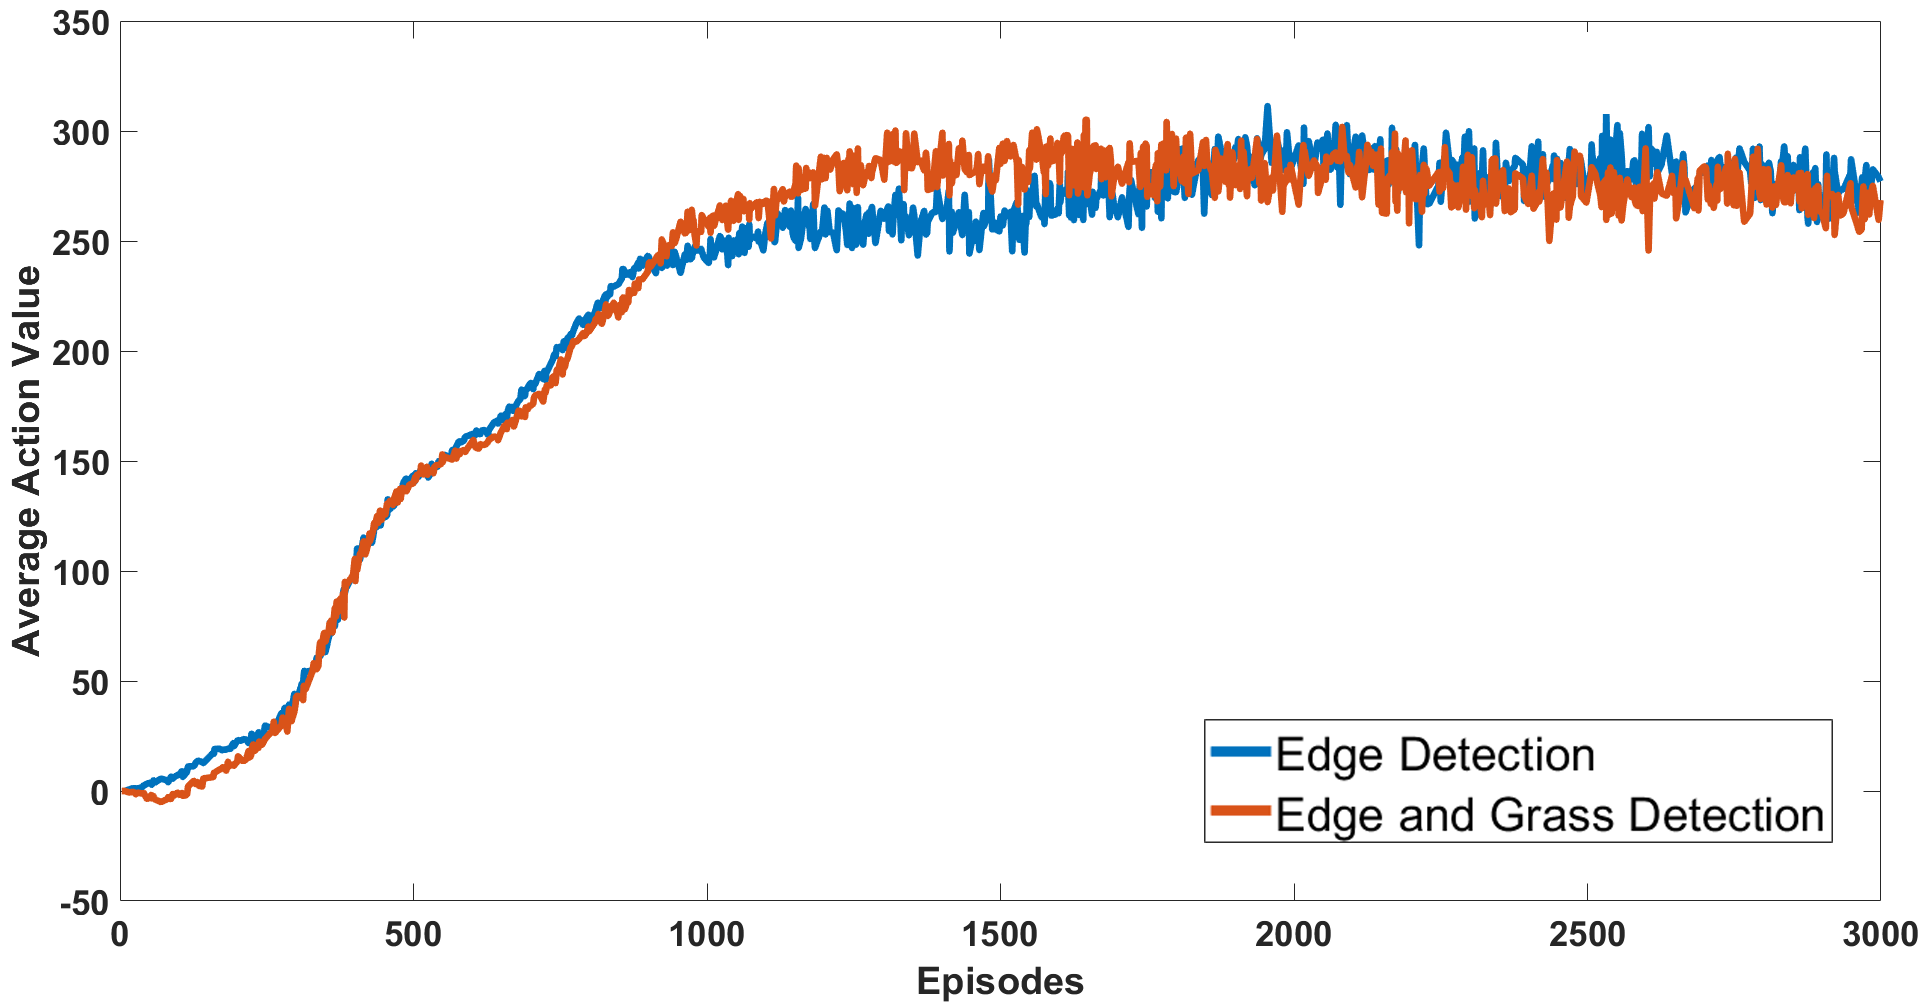
\includegraphics[width=.6\linewidth]{Graphics/grass_perf_q_large.png}
\caption{Average Q-value for grass detection}
\label{fig:grass_perf_q}
\end{figure}

\begin{figure}[h!]
\centering
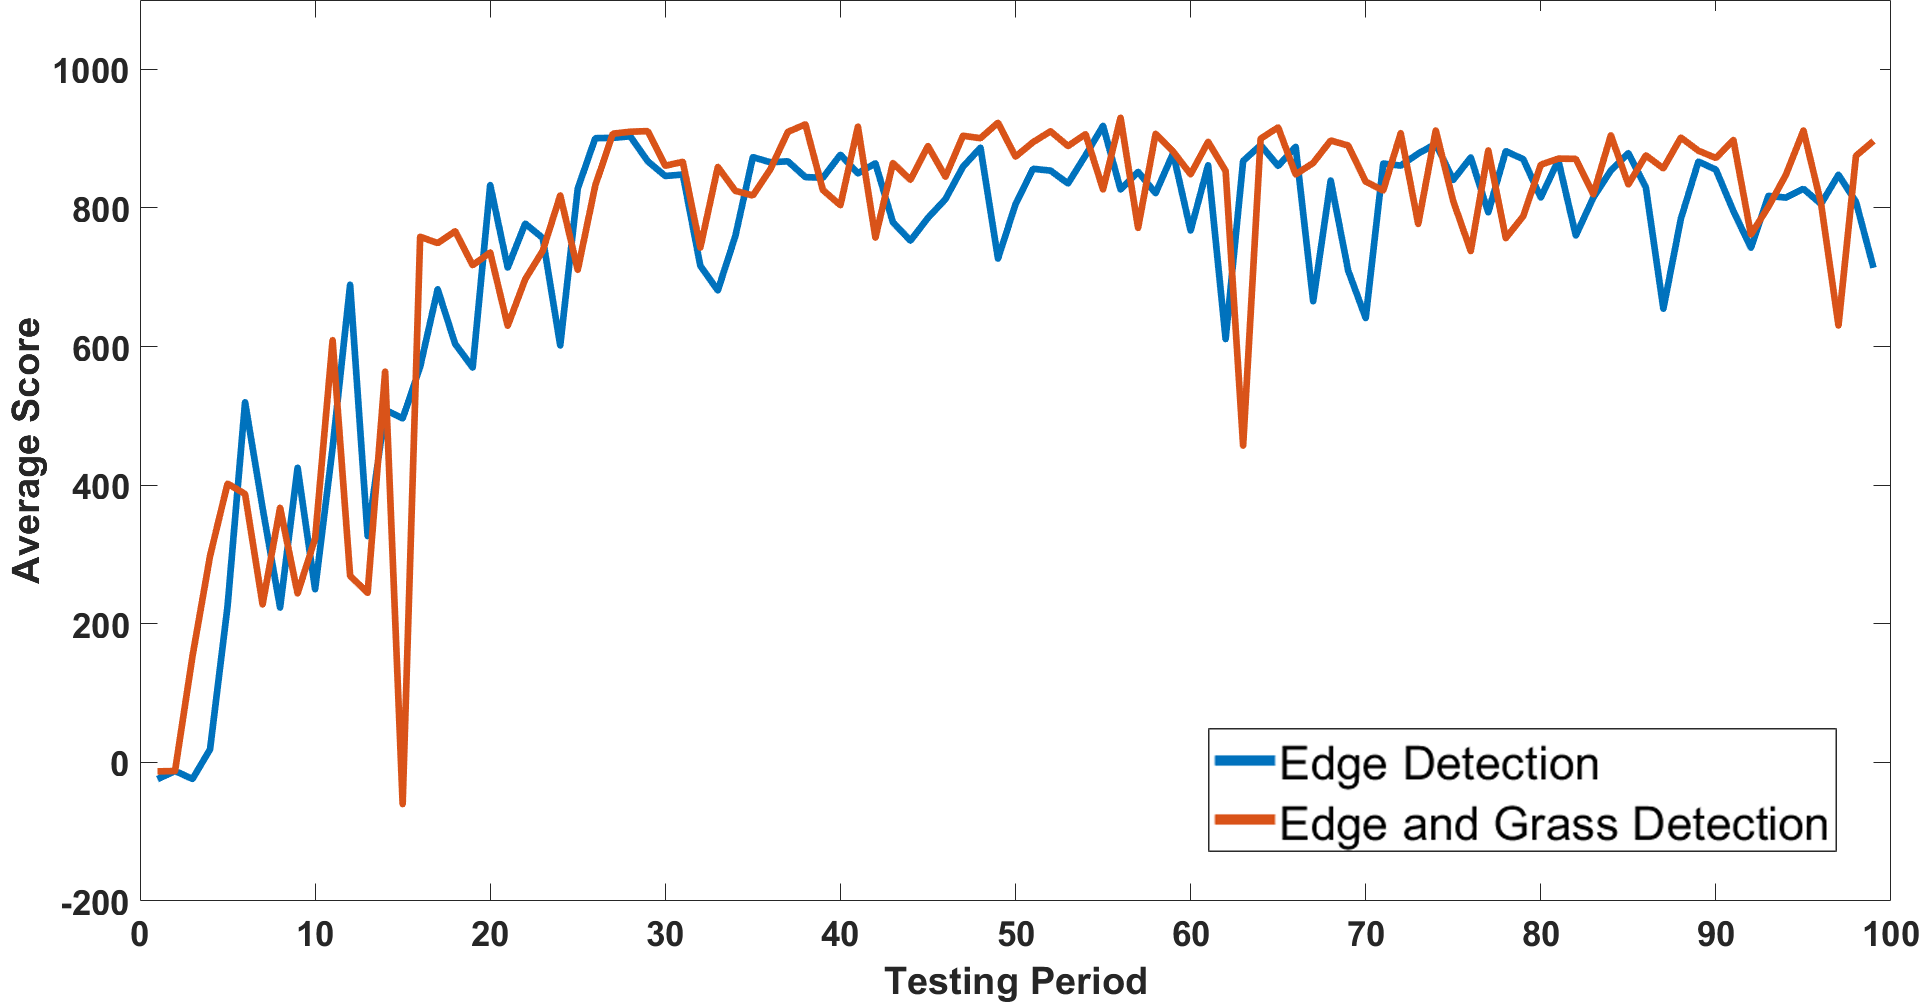
\includegraphics[width=.6\linewidth]{Graphics/grass_perf_score_large.png}
\caption{Average training score for grass detection}
\label{fig:grass_perf_score}
\end{figure}

As shown in Figure \ref{fig:grass_perf_q}, the average Q-value for
edge detection and edge with grass detection converge to the same values.
More importantly, as shown in Figure \ref{fig:grass_perf_score}, the training score
when using grass detection increases as compared to using edge detection
without grass detection. While both methods are able to exceed score of 
900, adding grass detection allows the agent to exceed the score more often
and reduces the number of times the car cuts corners. 

Our grass detection algorithm simply alters the reward function while 
training: it returns a score of -1 every time the car enters the grass.
In the context of real-world autonomous driving, grass detection can be 
interpreted as the auxiliary devices of the car. For example, the reward
given to the car while training can vary based on the distance between
the car and the sidewalk calculated with a radar.
Ultimately, 
incorporating grass detection into our algorithm while training, and
observing its performance on random tracks, suggests that 
such auxiliary data does not compromise the generalizability of our 
algorithm and improves its performance. 


\endinput







% Chapter 7
\ifthenelse{\boolean{@twoside}}{\myclearpage}{}
\chapter{Discussion}\label{Ch:FutureWork}

Our work has shown that the DQN algorithm does generalize from limited training environments to all tracks in the OpenAi CarRacing environment, but not perfectly. The algorithm fails occasionally during testing, such as cutting corners and swirling out of the road. There is still much work to do to uncover the reasons for these problems. We have compiled a list of ideas that could  improve the performance on this specific task, with some of them also applicable to other reinforcement learning problems:
\begin{itemize}
\item Explore hyperparameters more thoroughly, most importantly  replay memory size, batch size and update frequency for target Q-network
\item Explore multiple regularization methods and their hyperparameters
\item Try Deeper architectures
\item Introduce perturbations into the testing environment and analyze the effect
\end{itemize}

Nonetheless, we have surpassed the current score for the car racing game on the OpenAI leaderboard and come very close to solving the game. Our results involving dropout also shone some light on the positive effect regularization can have on Deep Reinforcement Learning algorithms.

\endinput



% Chapter 9 -- the Conclusion
% \ifthenelse{\boolean{@twoside}}{\myclearpage}{}
% \include{chapter9}

% Insert text in Table of Contents to highlight the appendix(es)
\addtocontents {toc}{\protect \contentsline {chapter}{APPENDIXES}{}}
\appendix
\ifthenelse{\boolean{@twoside}}{\myclearpage}{}
\chapter{Algorithms Outline}\label{Algorithms}
\section{Basic Q-Learning Algorithm Outline}
\begin{algorithm}[H]
 Initialize $Q(s,a)$ for all $s \in S, \;\; a \in A$\\
 \For{each episode}{
 Get initial state $s_t$\\
 \While{episode is not over}{
	Sample $U \sim Unif(0,1)$ \\
	\eIf{$U < \epsilon$}{
		$a_{t} =  \textrm{random action}$
	}{
	  	$a_{t} =  \underset{a'}\argmax \; Q(s_t,a')$
	}
	Take action $a_t$, get reward $R_{t+1}$ and new state $s_{t+1}$ \\
	Set
		$Q(s_t, a_t) = Q(s_t,a_t) +  \alpha\left(R_{{t+1}} + \gamma\;\underset{a'}\max \; Q(s_{t+1},a') - Q(s_t, a_t)\right)$\\
	$\; s_t = s_{t+1}$
 }
 }
 \caption{Basic Q-learning}
 \label{alg:basic_q}
\end{algorithm}

\newpage
\section{Deep Q-Learning Algorithm Outline}
\begin{algorithm}[H]
Initialise $Q$ with random weights $\theta$\\
Set $\theta^- = \theta$. \\
 \For{each episode}{
 Get initial state $s_0$\\
	 \For{t = 1, 2, 3 ... T}{
		Sample $U \sim Unif(0,1)$ \\
		Set $a_t = \begin{dcases}
		    \text{random action sampled uniformly} & \text{if U $< \epsilon$}\\
		    \underset{a'}\argmax \; Q(s_t,a')              & \text{otherwise}
		\end{dcases}$ \\
		Take action $a_t$, get reward $R_{t+1}$ and new state $s_{t+1}$ \\
		Store $(s_t, a_t, R_{t+1}, s_{t+1})$ in the replay memory $\mathcal{D}$\\
		Sample a random minibatch of transitions $(s_j, a_j, R_{j+1}, s_{j+1})$ from $\mathcal{D}$\\
		Set $y_j = \begin{dcases}
		    R_{j+1} + \gamma\, \max\limits_{a'} Q(s_{j+1}, a';\theta^-)& \text{if $s_{j+1}$ is not terminal} \\
		    R_{j+1},              & \text{otherwise}
		\end{dcases}$ \\
		Perform a gradient descent step on the loss $\left( y_j - Q(s_j, a_j;\theta)\right)^2$ \\
		Every C steps set $\theta^- = \theta$. 
 	}
 }
\caption{Deep Q-learning}
\label{alg:deep_q}
\end{algorithm}

\endinput

\ifthenelse{\boolean{@twoside}}{\myclearpage}{}
\chapter{Parameters}\label{Parameters}

\section{Neural Network Structures}
\begin{table}[h!]
\begin{center}
\begin{tabular}{| l | l | l|}
\hline
Layer Number & Two Convolutional Layers & Three Convolutional Layers\\
\hline
Layer 1 & Convolutional, 16 8x8 kernels with stride 4, 
ReLU activiation & Convolutional, 32 8x8 kernels with stride 4, 
ReLU activiation\\
\hline
Layer 2 & Convolutional, 32 4x4 kernels with stride 2, 
ReLU activiation & Convolutional, 64 4x4 kernels with stride 2, 
ReLU activiation\\
\hline
Layer 3 & Dense, 256 kernels, ReLU activiation & Convolutional, 64 3x3 kernels with stride 1, ReLU activiation\\
\hline
Layer 4 & Dense, 5 kernels, linear activation & Dense, 512 kernels, ReLU activation\\
\hline
Layer 5 &  & Dense, 5 kernels, linear activation\\
\hline
\end{tabular}
\caption{Neural Network Structures}
\label{table: neuralstructures}
\end{center}
\end{table}

\section{Actions}
\begin{table}[h!]
\begin{center}
\begin{tabular}{| l | l|}
\hline
Four Actions & Five Actions\\
\hline
Left Turn [-1, 0, 0] & Left Turn [-1, 0, 0]\\
\hline
Right Turn [1, 0, 0] & Right Turn [1, 0, 0]\\
\hline
Acceleration [0, 1, 0] & Acceleration [0, 1, 0]\\
\hline
Deceleration [0, 0, 0.8] & Deceleration [0, 0, 0.8]\\
\hline
 & No Operation [0, 0, 0]\\
\hline
\end{tabular}
\caption{Action Space Comparison}
\label{table: ActionSpace}
\end{center}
\end{table}

\section{Hyperparameters}
\begin{table}[h!]
\begin{center}
\begin{tabular}{ |c|c| } 
\hline
Name & Value \\
\hline
Architecture & Three convolutional layers\\
\hline
Explore Rate & Decrease from 1 to 0.1 linearly for the first 250000 frames, 0.1 thereafter\\
\hline
Learning Rate & 0.00025\\
\hline
Discount Rate & 0.99 \\
\hline
Batch Size & 32 \\
\hline
Memory Capacity & 100000 \\
\hline
\end{tabular}
\caption{Hyperparameters}
\label{table: hyperparameters}
\end{center}
\end{table}

\endinput

\ifthenelse{\boolean{@twoside}}{\myclearpage}{}
\chapter{Glossary}\label{Glossary}

\begin{table}[!h]  % Note override ("!") of normal placement algorithm to force placement on 1st page.
\begin{tabular}{ p{0.2\textwidth} p{0.75\textwidth} }

{\bf Agent}: &		Decision maker \\ \\

{\bf Environment}: & World the agent interacts with\\ \\

{\bf State}:  &  Snapshot of the environment e.g. a screenshot of the game (denoted as $S$)\\ \\

{\bf Action}: & Actions the agent can take, e.g. accelerate or turn right (denoted as $A$)\\ \\

{\bf Reward}: & Scalar feedback from environment to agent (denoted as $R$)\\ \\

{\bf Return}: & Sum of all rewards the agent receives (denoted as $\mathcal{R}$) \\ \\

{\bf Q-Learning}: & A reinforcement learning technique used in machine learning. \\ \\

{\bf Dropout}: & A common regularization technique. \\ \\

\end{tabular}
%\caption{A sample table used as a glossary.}
\end{table}

\endinput

\ifthenelse{\boolean{@twoside}}{\myclearpage}{}
\chapter{Abbreviations}\label{Abbreviations}

\noindent AI.  Artificial Intelligence.

\vspace{5pt}

\noindent DDQN.  Double Deep Q-Network.

\vspace{5pt}

\noindent DQN.  Deep Q-Network.

\vspace{5pt}

\noindent IPAM. Institute for Pure and Applied Mathematics.  An institute of the National Science  Foundation, located at UCLA.

\vspace{5pt}

\noindent MDP.  Markov Decision Process.

\vspace{5pt}

\noindent RGB (image).  Red, Green and Blue (image).

\vspace{5pt}

\noindent RIPS.  Research in Industrial Projects for Students.  A regular summer program at IPAM, in which teams of undergraduate (or fresh graduate) students participate in sponsored team research projects.

\vspace{5pt}

\noindent RL.  Reinforcement Learning.

\vspace{5pt}

\noindent RLP.  Reinforcement Learning Problem.

\vspace{5pt}

\noindent SGD.  Stochastic Gradient Descent.

\vspace{5pt}

\noindent TD.  Temporal Difference.

\vspace{5pt}

\noindent UCLA.  The University of California at Los Angeles.

\vspace{5pt}


\endinput

% Add your bibliography to Contents
\ifthenelse{\boolean{@twoside}}{\myclearpage}{\newpage}
\addtocontents {toc}{\protect \contentsline {chapter}{REFERENCES}{}}
\addcontentsline{toc}{chapter}{Reference}  % Use the 'bibname' name here.  See below.

% Bibliography must come last.
\bibliographystyle{siam}     % Siam and Ieeetr bibliographic styles treat titles of articles in journals or collections correctly
\renewcommand\bibname{References}
\nocite{*}  % List ALL references in your references, not just the ones cited in the text.
% This scheme automatically alphabetizes the Bibliography.
\bibliography{AA-Bibliography/RIPS_AMD}

\end{document}
